% THIS DOCUMENT IS FOLLOWS THE VOLERE TEMPLATE BY Suzanne Robertson
% and James Robertson
% ONLY THE SECTION HEADINGS ARE PROVIDED
%
% Initial draft from https://github.com/Dieblich/volere
%
% Risks are removed because they are covered by the Hazard Analysis
\documentclass[12pt]{article}

\usepackage[round]{natbib}
\usepackage[letterpaper, portrait, margin=1in]{geometry}
\usepackage{booktabs}
\usepackage{longtable}
\usepackage{siunitx}
\usepackage{tabularx}
\usepackage[dvipsnames]{xcolor}
\usepackage{hyperref}
\usepackage{enumitem}
\usepackage{graphicx}
\hypersetup{
  bookmarks=true,         % show bookmarks bar?
  colorlinks=true,      % false: boxed links; true: colored links
  linkcolor=red,          % color of internal links (change box color
  % with linkbordercolor)
  citecolor=green,        % color of links to bibliography
  filecolor=magenta,      % color of file links
  urlcolor=cyan           % color of external links
}
\usepackage{float}

\newcommand{\lips}{\textit{Insert your content here.}}

% Test line
% Test 2

%% Comments

\usepackage{color}

% \newif\ifcomments\commentstrue %displays comments
\newif\ifcomments\commentsfalse %so that comments do not display

\ifcomments
\newcommand{\authornote}[3]{\textcolor{#1}{[#3 ---#2]}}
\newcommand{\todo}[1]{\textcolor{red}{[TODO: #1]}}
\else
\newcommand{\authornote}[3]{}
\newcommand{\todo}[1]{}
\fi

\newcommand{\wss}[1]{\authornote{blue}{SS}{#1}} 
\newcommand{\plt}[1]{\authornote{magenta}{TPLT}{#1}} %For explanation of the template
\newcommand{\an}[1]{\authornote{cyan}{Author}{#1}}

%% Common Parts

\newcommand{\progname}{Software Engineering} % PUT YOUR PROGRAM NAME HERE
\newcommand{\authname}{\textbf{Team 4, EcoOptimizers} \\
  \\ Nivetha Kuruparan
  \\ Sevhena Walker
  \\ Tanveer Brar
  \\ Mya Hussain
\\ Ayushi Amin} % AUTHOR NAMES

\usepackage{hyperref}
\hypersetup{colorlinks=true, linkcolor=blue, citecolor=blue, filecolor=blue,
urlcolor=blue, unicode=false}
\urlstyle{same}



\begin{document}

\pagenumbering{roman}

\title{Software Requirements Specification for \progname: subtitle
describing software}
\author{\authname}
\date{\today}

\maketitle
\thispagestyle{empty}

~\newpage

\tableofcontents
% This is a test line, please ignore

~\newpage

\section*{Revision History}

\begin{tabularx}{\textwidth}{p{3.7cm}p{1.8cm}X}
  \toprule {\textbf{Date}} & {\textbf{Name}} & {\textbf{Notes}}\\
  \midrule
  October 11th, 2024 & All & Created initial revision of SRS\\
  January 2nd, 2025 & All & Added clarification to training requirements\\
  January 5th, 2025 & All & Update FR-7, FR-8, Ideas for Solution \\
  January 6th, 2025 & All & Fixed link references to tables and
  figures and added preambles to those sections, move glossary
  section, added symbolic constants\\
  February 8th, 2025 & All & Removed requirement for interfacing with
  GitHub Actions.\\
  February 10th, 2025 & All & Updated the data dictionary and
  business data model \\
  February 10th, 2025 & All & Updated costs, compliance requirements,
  security requirements and scope of the product. \\
  March 24th, 2025 & All & Updated and added functional requirements. \\
  March 24th, 2025 & Mya Hussain & Updated Usability and Humanity Requirements. \\
  March 24th, 2025 & Ayushi Amin & Updated maintainability and support requirements. \\
  March 24th, 2025 & Ayushi Amin & Updated cultural requirements.
  \bottomrule 
\end{tabularx}

~\\

~\newpage

\section*{Symbolic Constants}
\begin{table}[H]
  \centering
  \begin{tabular}{|l|c|}
    \toprule \textbf{Name} & \textbf{Value} \\
    \midrule
    ENERGY\_SAVE & 5\% \\
    SMELL\_COVERAGE & 80\% \\
    TEST\_FUNCTION\_THRESH & 100\% \\
    REFACTOR\_EFFICACY\_THRESH & 95\% \\
    REFACTOR\_REVERT\_LIMIT & 5 commits \\
    CRITICAL\_ENERGY\_SAVE\_THRESH & 10\% \\
    MIN\_USER\_CONFIDENCE & 70\% \\
    MAX\_TASK\_CLICKS & 4 clicks \\
    MIN\_USER\_EOU & 80\% \\
    SMALL\_FILE\_TIME & 5 sec \\
    LARGE\_FILE\_TIME & 30 sec \\
    REFACTOR\_TIME & 10 sec \\
    DETECTION\_ACC & 90\% \\
    LARGE\_CODE\_BASE\_TIME & 2 min \\
    NEW\_REFACTOR\_TIME & 7 days \\
    COMPREHENSION\_TIME & 2 days \\
    ROLLBACK\_TIME & 1h \\
    MIN\_CODE\_COVERAGE & 80\% \\
    OS\_PERF\_DIFF\_LIMIT & 5\% \\
    \bottomrule
  \end{tabular}
  \caption{Table of Symbolic Constants}
  \label{tab:syms}
\end{table}

~\\

~\newpage

\pagenumbering{arabic}

\section{Purpose of the Project}
\subsection{User Business}
The Information and Communications Technology (ICT) sector, an
essential component of the global economy, is responsible for 2-4\%
of global CO2 emissions today, with projections suggesting this could
rise to 14\% by 2040 ~\citep{BelkhirAndElmeligi2018}. To meet
sustainability goals, including a 72\% reduction in CO2 emissions by
2040 ~\citep{FreitagAndBernersLee2021}, this sector must find ways to
improve energy efficiency.

One area of concern is the energy consumption of software systems.
However, for software engineers, it is not practical for them to
focus on optimizing energy consumption while developing complex
programs. Instead, supporting tools and technologies are needed to
assist in improving energy efficiency without altering the intended
behaviour of the software.

This project aims to tackle Python, a popular but energy inefficient
programming language. Python consumes significantly more energy
compared to more efficient languages like C and Rust—over 70 times
more energy, on average, for similar tasks ~\citep{PereiraEtAl2017}.
The project's goal is to develop tools to reduce Python's energy
consumption through automated refactoring. While this will not solve
the entire problem of the carbon footprint associated with the
software, it is a step towards more energy-efficient practices in the
software development process.

\subsection{Goals of the Project}
\noindent \textbf{Purpose}: The purpose of this project is to provide
software engineers with tools to optimize the energy efficiency of
Python programs by automating refactoring suggestions, while still
allowing users to review and decide whether to apply the changes.

\noindent \textbf{Advantage}: By reducing the energy consumption of
Python programs, this project will contribute to the broader effort
of decreasing the carbon footprint of software development,
supporting the ICT sector's goal of reducing CO2 emissions by 72\% by
2040 ~\citep{FreitagAndBernersLee2021}.

\noindent \textbf{Measurement}: The project's success can be measured
by the reduction in energy usage
achieved after applying the refactorings. Benchmarks will compare the
energy consumption of original
and refactored code, to achieve a measurable percentage reduction in
energy consumption.

\section{Naming Conventions and Terminology}
\subsection{Glossary of All Terms, Including Acronyms, Used by Stakeholders
involved in the Project}

% --- TERMS PRESENT IN THE STAKEHOLDER SECTION ---
\paragraph*{supervisor}
A member of faculty from McMaster University responsible for
overseeing a project being worked on by students taking the SFWRENG
4G06 Capstone course.

\paragraph*{large-scale applications}
Applications that manage high volumes of data, users, or
transactions, typically requiring scalable architectures.

\paragraph*{cloud-hosted applications}
Software applications deployed and run on remote cloud servers,
accessible over the internet.

\paragraph*{environmental footprint}
The total impact an activity or product has on the environment,
measured by metrics like carbon emissions and resource consumption.

\paragraph*{refactoring}
The process of restructuring existing code without changing its
external behaviour to improve readability, performance, or maintainability.

\paragraph*{mobile environment}
A software environment specifically designed for mobile devices, such
as smartphones or tablets, which have limited resources.

\paragraph*{embedded environment}
A software environment where applications run on specialized hardware
with constrained resources, often without traditional operating systems.

\paragraph*{SaaS}
Software as a Service (SaaS) refers to cloud-based software
applications delivered to users via the internet on a subscription basis.

\paragraph*{backend}
The part of a software system that handles server-side logic,
database interactions, and application functionality not directly
visible to users.

\paragraph*{software developer}
A professional who designs, writes, and maintains software
applications or systems.

\paragraph*{data analyst}
A professional who processes and analyzes large sets of data to help
organizations make informed decisions.

\paragraph*{tech company}
A company focused on technology products and services, including
software, hardware, and IT services.

\paragraph*{freelance}
Self-employed individuals who offer specialized services, such as
software development, without long-term commitments to any employer.

\paragraph*{usability testing}
A method of evaluating how easy and user-friendly a software
application or product is by observing real users interacting with it.

% --- TERMS PRESENT IN THE OPERATIONAL AND ENVIRONMENTAL REQUIREMENTS
% SECTION ---
\paragraph*{Python Code}
Refers to the original Python code given by the end user to refactor.

\paragraph*{Refactored Code}
Refers to the Python code that had refactorings made to it.

\paragraph*{library}
A collection of pre-written code that developers can reuse in their
projects to add specific functionalities.

\paragraph*{Git}
\label{term:git}
A distributed version control system that allows multiple developers
to track changes in source code, collaborate, and manage project
history efficiently.

\paragraph*{GitHub}
\label{term:GitH}
A web-based platform used for version control and collaboration on
code through \hyperref[term:git]{Git} repositories.

\paragraph*{Actions}
A \hyperref[term:GitH]{GitHub} feature that automates tasks such as
testing, deployment, and continuous integration via custom workflows.

\paragraph*{workflow}
A sequence of automated steps or actions that define a process, often
for continuous integration, deployment, or testing.

\paragraph*{Visual Studio Code}
\label{term:VSC}
A free, open-source code editor developed by Microsoft, known for its
versatility and wide range of extensions.

\paragraph*{VS Code}
An abbreviation of \hyperref[term:VSC]{Visual Studio Code}

\paragraph*{Visual Studio Code (VS Code) marketplace}
An online platform where users can discover, install, and manage
extensions that enhance the functionality of
\hyperref[term:VSC]{Visual Studio Code}.

\paragraph*{JSON}
\label{term:JSON}
\hyperref[term:JS]{JavaScript} Object Notation, a lightweight data
format used to store and exchange information between systems.

\paragraph*{XML}
\label{term:XML}
Extensible Markup Language, a data format used to encode documents in
a way that is both human-readable and machine-readable.

\paragraph*{package manager}
A tool that automates the process of installing, updating, and
managing software packages or libraries in a project.

\paragraph*{PIP}
A package manager for \hyperref[term:python]{Python} that simplifies
the installation and management of Python libraries.

% --- TERMS PRESENT IN WAITING ROOM SECTION ---
\paragraph*{IDE}
Integrated Development Environment, a software application providing
tools like a code editor, debugger, and compiler to facilitate development.

\paragraph*{progress indicators}
Visual or textual cues, such as loading bars or percentages, that
inform users about the status of ongoing processes.

\paragraph*{plugin}
A software component that adds specific features or functionalities
to an existing software system.

\paragraph*{configuration file}
A file used to define settings or preferences for a software
application, often stored in a human-readable format like
\hyperref[term:JSON]{JSON} or \hyperref[term:XML]{XML}.

\paragraph*{dashboard}
A user interface that provides an overview of key information and
metrics, typically presented in graphs, charts, and tables.

\paragraph*{sync}
The process of ensuring that data is consistent across multiple
systems or devices by automatically updating changes in real-time.

\paragraph*{programming language}
\label{term:progl}
A formal language used to write software programs by providing
instructions that a computer can execute.

\paragraph*{Python}
\label{term:python}
A \hyperref[term:progl]{programming language} known for its
simplicity and versatility, widely used in web development, data
science, and automation.

\paragraph*{Java}
A \hyperref[term:progl]{programming language} known for its
portability and scalability, commonly used for enterprise-level applications.

\paragraph*{C/C++}
A \hyperref[term:progl]{programming language} family used for system
programming, game development, and applications requiring high performance.

\paragraph*{C\#}
A \hyperref[term:progl]{programming language} developed by Microsoft,
primarily used for developing applications on the .NET platform.

\paragraph*{JavaScript}
\label{term:JS}
A \hyperref[term:progl]{programming language} used primarily for
adding interactivity to web pages and building dynamic web applications.

\paragraph*{TypeScript}
A \hyperref[term:progl]{programming language} that builds on
JavaScript by adding static typing, improving code reliability and scalability.

\paragraph*{Go}
A \hyperref[term:progl]{programming language} created by Google,
designed for simplicity and efficiency in building scalable applications.

\paragraph*{Rust}
A \hyperref[term:progl]{programming language} focused on safety,
performance, and concurrency, often used in system programming.

\section{Stakeholders}

The stakeholders involved in this project include all individuals and
groups that have a direct or indirect interest in the development,
implementation, and usage of the refactoring library for energy
efficiency. These stakeholders influence project decisions and will
be impacted by their outcomes. Understanding their roles and
expectations is crucial for ensuring that the library meets the needs
of its users and aligns with broader organizational goals.\\

This section introduces the \textbf{client}, \textbf{customer}, and
\textbf{other stakeholders} that are involved in the project.
Finally, we will look at the users of the product, specifically the
\textbf{hands-on-users}, what their \textbf{personas} may look like,
their \textbf{priority} levels, and what kind of
\textbf{participation} we can expect from them throughout the
development of this product.
\subsection{Client}
The client of this project is \textbf{Dr. Istvan David} from
McMaster's Department of Computing and Software. As the project
supervisor, his role is to guide the development team with his
technical and domain expertise. As the client, he sets the product's
requirements and will be involved throughout its development.
\subsection{Customer}
The customers of this product are \textbf{software developers}.
Specifically, they are the developers that work in teams for small to
large corporations, or freelancers looking to improve their services.
They will be the primary users of the product and, therefore, will
offer critical feedback on its effectiveness such as suggestions for
improvement and/or additional features. Any feedback received from
this stakeholder will be given top priority for consideration as the
goal for this tool is to be an integral part of a software developer's workflow.

\subsection{Other Stakeholders}
\subsubsection*{\textcolor{Maroon}{Project Managers}}
They oversee project operations and focus on reducing energy costs
associated with large-scale or cloud-hosted applications. They might
leverage the refactoring library to reduce operational costs and
achieve business sustainability goals.

\subsubsection*{\textcolor{Maroon}{Business Sustainability Teams}}
This stakeholder is responsible for reducing the company's
environmental footprint by analyzing its energy emissions. They will
use the energy efficiency metrics provided by the refactoring library
to improve environmental sustainability practices within their organization.

\subsubsection*{\textcolor{Maroon}{End Users}}
End users refer to the users of software that uses the product in its
development. They will indirectly reap benefits from these
applications that have been optimized using the refactoring library.
Software used, especially mobile or embedded environments where
battery life is a key concern, might prove to be more responsive and
efficient. They have no involvement in the development of the product.

\subsubsection*{\textcolor{Maroon}{Regulatory Bodies}}
This stakeholder is responsible for establishing regulations
governing energy consumption and sustainability standards. They can
promote the adoption of energy-efficient software practices and
potentially certify tools that meet regulatory standards.

\subsection{Hands-On Users of the Project}
\subsubsection*{\textcolor{Maroon}{Software Developers}}
\begin{itemize}
  \item \textbf{User Role}: Integrate library into the codebase,
    provide tests to check refactoring against original functionality

  \item \textbf{Subject Matter Experience}: Journeyman to Master

  \item \textbf{Technological Experience}: Journeyman to Master

  \item \textbf{Attitude toward technology}: Varies (conservative to positive)

  \item \textbf{Physical location}: Remote (at home), in-person (work
    office) or hybrid
\end{itemize}

\subsubsection*{\textcolor{Maroon}{Business Sustainability Teams}}
\begin{itemize}
  \item \textbf{User Role}: Access metrics provided by library

  \item \textbf{Subject Matter Experience}: Journeyman

  \item \textbf{Technological Experience}: Novice to Journeyman

  \item \textbf{Attitude toward technology}: Neutral to positive

\end{itemize}

\subsection{Personas}

\subsubsection*{Persona: Raven Reyes}
\textbf{Age:} 37\\
\textbf{Job Title:} Senior Software Developer\\
\textbf{Education:} Bachelor's in Computer
Science\\[2mm]
\textbf{Work Environment:} Works at a mid-sized SaaS company with a
focus on improving their environmental footprint.\\
\textbf{Professional Background:} Has over 15 years of experience in
software development, specializing in backend systems. Worked with
various programming languages (Python, Java, and C++), and is
well-versed in optimizing code for performance.\\[2mm]
\textbf{Need:} With the company more focused on sustainability, Raven
and her team need to go through their codebase and apply energy
efficient changes to their code.\\
\textbf{Challenges:} Knowing what to change in their code to make it
more efficient is challenging, not to mention the incredible amount
of code they will have to sift through. We are talking hundreds of
thousands of lines of code!

\subsubsection*{Persona: Christopher Robin}
\textbf{Age:} 34\\
\textbf{Job Title:} Data Analyst\\
\textbf{Education:} Bachelor's in Data Science\\[2mm]
\textbf{Work Environment:} Works at a large corporation that has
recently started increasing their efforts to become a sustainable company.\\
\textbf{Professional Background:} Over 8 years of experience in data
analysis, just recently looking into sustainability metrics.
Christopher regularly collaborates with IT teams to track performance
metrics and recently energy consumption metrics to help identify
areas for improvement.\\[2mm]
\textbf{Need:} Christopher needs accurate data on energy consumption
from the company's software systems to generate insights that drive
sustainability initiatives and help meet corporate environmental targets.\\
\textbf{Challenges:} Translating raw technical data into meaningful
insights that can guide decisions is difficult, especially when
working with complex systems.

\subsubsection*{Persona: Draco Malfoy}
\textbf{Age:} 29\\
\textbf{Job Title:} Freelance Software Developer\\
\textbf{Education:} Bachelor's in Software Engineering\\[2mm]
\textbf{Work Environment:} Works remotely on multiple freelance
projects for small and mid-sized businesses, focusing on web
applications and backend systems.\\
\textbf{Professional Background:} Has 7 years of experience working
with various clients to develop and optimize software, primarily in
Python and JavaScript. He often works on tight deadlines, where
balancing performance and development speed is key.\\[2mm]
\textbf{Need:} Draco needs efficient ways to optimize the code he
writes for clients, particularly in terms of performance and energy
efficiency, as more businesses become environmentally conscious.\\
\textbf{Challenges:} As a freelancer, time is money. Draco needs
tools that help him quickly identify inefficiencies in the code and
refactor them, without spending hours analyzing large codebases or
learning new systems.

\subsection{Priorities Assigned to Users}
\textbf{Key Users:} Software Developers, Business Sustainability Teams \\
\textbf{Secondary User:} Project Managers

\subsection{User Participation}
For the bulk of the development process, requirements will be
gathered from the development team itself with the help of the
project supervisor, Dr. Istvan David.

During the testing phase, usability testing will be conducted to
further refine the product.

\subsection{Maintenance Users and Service Technicians}
Due to the nature of this project as a capstone requirement, there
are currently no expected maintenance users.

\section{Mandated Constraints}
\subsection{Solution Constraints}
\begin{enumerate}[label=MD-SL \arabic*., wide=0pt, leftmargin=*]
  \item \emph{The system must refactor Python code without changing
    its original functionality.}\\[2mm]
    {\bf Rationale:} The project is focused on energy-efficient
    refactoring for Python code, and altering functionality could
    break existing software behaviour.\\
    {\bf Fit Criterion:} The system must pass all original test cases
    after refactoring, ensuring that functionality remains unchanged.\\
    {\bf Priority:} High
  \item \emph{The refactored code must result in measurable energy
    savings.}\\[2mm]
    {\bf Rationale:} The project's primary objective is to improve
    the code's energy efficiency. Refactorings should lead to a
    noticeable reduction in energy consumption.\\
    {\bf Fit Criterion:} The system must show at least a ENERGY\_SAVE
    reduction in energy consumption, as measured by tools like
    \texttt{CodeCarbon}, for most of the refactored code.\\
    {\bf Priority:} High
  \item \emph{The refactored code must be provided to the user upon
    completion of the refactoring process.}\\[2mm]
    {\bf Rationale:} Developers need access to the refactored code to
    utilize it in their projects immediately after the refactoring process.\\
    {\bf Fit Criterion:} The system must deliver the refactored code
    to the user in a clear format, ensuring it is readily available
    for implementation.\\
    {\bf Priority:} High
\end{enumerate}

\subsection{Implementation Environment of the Current System}
\begin{enumerate}[label=MD-EC \arabic*., wide=0pt, leftmargin=*]
  \item \emph{The product shall be able to run on standard laptop
      environments, including typical developer setups with operating
    systems such as Windows, macOS, and Linux.}\\[2mm]
    {\bf Rationale:} Developers will primarily use the tool on
    personal workstations, including laptops, and it must integrate
    smoothly with typical development environments. Supporting
    standard laptop environments ensures that the tool is accessible
    to a wide range of users without the need for specialized hardware.\\
    {\bf Fit Criterion:} The tool must be installable and functional
    on a standard laptop with Visual Studio Code. It should perform
    well without requiring excessive processing power or memory.\\
    {\bf Priority:} High
\end{enumerate}
\subsection{Partner or Collaborative Applications}
The project will focus on developing the tool with flexibility for
integration with Visual Studio Code. While no specific partner
applications are required, understanding these possibilities can aid
smoother integration. Future collaboration with Python development
tools may be considered, but no formal interface constraints are
needed at this stage.
\subsection{Off-the-Shelf Software}
The project has no strict requirements for off-the-shelf software but
will leverage open-source libraries to enhance functionality and
maintain flexibility. Tools like CodeCarbon for energy measurement
and Python analysis libraries may be used. While no legal issues are
expected, all tools will be assessed for compatibility. Documentation
will be maintained, though no specific constraints are set at this stage.
\subsection{Anticipated Workplace Environment}
The workplace will include standard software development setups. The
tool should offer a non-intrusive interface suited for quiet
workspaces and providing quick feedback in collaborative environments.
\subsection{Schedule Constraints}
\begin{enumerate}[label=SCHD \arabic*., wide=0pt, leftmargin=*]
  \item \emph{The project shall be completed by April 2025, with
      interim deadlines for key milestones such as Proof of Concept
    (November 2024) and the final demonstration (March 2025).}\\[2mm]
    {\bf Rationale:} These deadlines are based on the academic
    timeline and the expectations of the capstone course.\\
    {\bf Fit Criterion:} All project components must be completed and
    fully functional by the final demonstration in March 2025.\\
    {\bf Priority:} High
\end{enumerate}
\subsection{Budget Constraints}
\begin{enumerate}[label=BDGT \arabic*., wide=0pt, leftmargin=*]
  \item \emph{The project shall not exceed the resources available to
      the team, which includes free open-source software and free
    services like GitHub for hosting.}\\[2mm]
    {\bf Rationale:} The team does not have a budget for paid
    services or proprietary software.\\
    {\bf Fit Criterion:} The project must be implemented using free
    tools and libraries and hosted on GitHub.\\
    {\bf Priority:} High
\end{enumerate}
\subsection{Enterprise Constraints}
\begin{enumerate}[label=ENTP \arabic*., wide=0pt, leftmargin=*]
  \item \emph{The product shall be built to comply with the standards
      of McMaster University’s capstone project requirements and
    academic integrity policies.}\\[2mm]
    {\bf Rationale:} The project is part of the university’s
    curriculum and must adhere to its standards.\\
    {\bf Fit Criterion:} The product must meet the requirements
    specified by the course syllabus and project advisor.\\
    {\bf Priority:} High
\end{enumerate}

\section{Relevant Facts And Assumptions}
\subsection{Relevant Facts}
Not applicable to this system.
\subsection{Business Rules}

The following are some business rules established between the team.

\begin{enumerate}
  \item \textbf{Project Timeline Adherence:} All milestones must be
    completed according to the established project timeline. Any
    delays or unexpected circumstances must be reported to the team
    as soon as possible.
  \item \textbf{Pull Request Review Requirement:} All pull requests
    must receive at least two independent reviews before they can be
    merged into the main branch. Reviewers must provide feedback or
    approval within 48 hours of the request to ensure timely progress.
  \item \textbf{Team Communication Standard:} All team members are
    required to communicate in a friendly and respectful manner
    during discussions, meetings, and in all written communications.
    Constructive feedback should be provided with the intent to
    support and enhance team collaboration.
\end{enumerate}

\subsection{Assumptions}
It is assumed for this system that users will be seeking to refactor
Python code and will make use of Visual Studio Code.

\section{The Scope of the Work}
This section defines the boundaries and objectives of the work,
focusing on the tasks and components required to develop and deliver
the refactoring library. It provides a clear view of how the system
operates within its context and breaks the work into logical
partitions to facilitate development and implementation.

\subsection{The Current Situation}

The current software development landscape often prioritizes
functionality and performance over energy efficiency. Many existing
Python codebases are not optimized for energy consumption, leading to
unnecessary power usage and increased carbon footprint. The following
aspects characterize the current situation:
\begin{enumerate}
  \item \textbf{Manual Refactoring:} Developers typically perform
    refactoring manually, which is time-consuming and prone to errors.
  \item \textbf{Limited Awareness:} Many developers lack awareness of
    energy-efficient coding practices and their impact on overall
    energy consumption.
  \item \textbf{Absence of Automated Tools:} There is a lack of
    widely adopted automated tools specifically designed to refactor
    Python code for energy efficiency.
  \item \textbf{Performance-Centric Optimization:} Most existing
    optimization tools focus on performance improvements rather than
    energy efficiency.
  \item \textbf{Inefficient Code Patterns:} Many codebases contain
    inefficient code patterns that consume more energy than necessary.
\end{enumerate}

\textcolor{red}{The project aims to address these issues by:}
\begin{enumerate}
  \item \textbf{Automated Refactoring Library:} Developing a Python
    library that automatically detects and refactors code for
    improved energy efficiency.
  \item \textbf{IDE Integration:} Creating a Visual Studio Code
    plugin that integrates the refactoring library, providing
    real-time suggestions and automated refactoring options.
  \item \textbf{Energy Consumption Measurement:} Implementing tools
    to measure and compare energy consumption before and after refactoring.
  \item \textbf{Developer Education:} Raising awareness about
    energy-efficient coding practices through the tool's suggestions
    and documentation.
  \item \textbf{Continuous Improvement:} Implementing a reinforcement
    learning model to improve refactoring suggestions over time based
    on developer feedback and real-world energy savings data.
\end{enumerate}

\subsection{The Context of the Work}
The purpose of this subsection is to illustrate the flow of inputs,
outputs, and interactions between the refactoring library and its
external systems, such as developers, energy measurement tools, and
machine learning frameworks. \hyperref[img:work-context]{Figure 1}
highlights the connections between the system's components and
external elements, ensuring a comprehensive understanding of its
operational environment.

\begin{figure}[H]
  \centering
  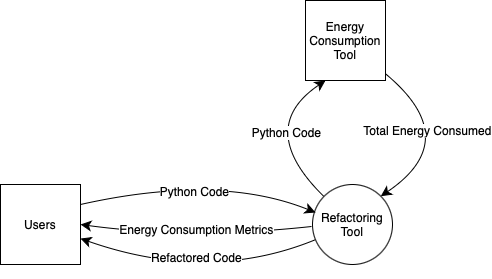
\includegraphics[scale=0.5]{../Images/WorkContextModel.png}
  \caption{Work Context Diagram}
  \label{img:work-context}
\end{figure}

\newpage
\subsection{Work Partitioning}
In this subsection, the work needed to complete this system is
divided into distinct activities, such as identifying code smells,
applying refactorings, and measuring energy efficiency. As seen in
\hyperref[tab:work-part]{Table 2}, each partition outlines its
purpose, dependencies, and deliverables to provide a structured
overview of the project's tasks.

\begin{table}[H]
  \centering
  \setlength\extrarowheight{5mm}
  \begin{tabularx}{\textwidth}{|c|X|l|p{1.5in}|}
    \toprule \textbf{Event \#} & \textbf{Event Name} & \textbf{Input}
    & \textbf{Output(s)} \\
    \midrule
    1 & Users submit Python code & Python Code & Refactored Code\\
    2 & Energy Analysis of code & Python Code & Total Energy Consumed \\
    3 & RI Model produces refactoring & Python Code & Correct Refactoring \\
    4 & Testing and Validation of refactored code & Refactored Code &
    Test Results \\
    5 & Reporting Performance metrics of new code & Refactored Code &
    Performance Reports \\
    6 & Viewing Energy consumption reports & Refactored Code & Energy
    Consumption Statistics \\
    \bottomrule
  \end{tabularx}
  \caption{Work Partitioning of System}
  \label{tab:work-part}
\end{table}

\subsection{Specifying a Business Use Case (BUC)}
Each event listed in \hyperref[tab:work-part]{Table 2} is expanded
into an individual business use case which describes how the system
handles specific scenarios.

\begin{enumerate}[label={\bf BUC \arabic*:}, wide=0pt, font=\itshape]
  \item {\bf Code Submission} \\[2mm]
    \textbf{Input:} Python Code \\
    \textbf{Output:} Refactored Code \\
    \textbf{Pre-condition:} User uses either GitHub Action or a VS
    Code plugin to submit code to the refactoring tool \\[2mm]
    \textbf{Scenario:}
    \begin{enumerate}[label=\arabic*.]
      \item Refactoring tool receives the Python code
      \item PyJoules is used to store energy consumption data for the
        original Python code submitted
      \item Tool analyzes the code for inefficiencies (PySmells)
      \item Python code is provided to the Re-enforcement learning
        model to find a refactoring
      \item Energy consumption is measured of refactored code and
        compared to the original data
      \item Refactored code is tested to ensure functionality is
        maintained from the original code
      \item Refactored code is received by the user
    \end{enumerate}
    \textbf{Sub Variation: }
    \begin{itemize}
      \item \textit{4a:} If no PySmells are identified, then code is
        returned to the user
      \item \textit{6a:} If energy consumption increases for
        refactored code, the reinforcement model is asked to find
        another refactoring
      \item \textit{7a:} If code functionality is not preserved for
        refactored code, the reinforcement model is asked to find
        another refactoring
    \end{itemize}

  \item {\bf Energy Analysis of Code}\\[2mm]
    \textbf{Input:} Python Code \\
    \textbf{Output:} Total Energy Consumed \\
    \textbf{Pre-condition:} Submission of Python code to the Energy
    Consumption Tool \\[2mm]
    \textbf{Scenario: }
    \begin{enumerate}[label=\arabic*.]
      \item Tool receives Python Code
      \item Energy consumed is measured during execution
      \item The analysis results are compiled into a report
      \item Report of total energy consumed is received by the refactoring tool
    \end{enumerate}

  \item {\bf Reinforcement Learning Model Produces Refactoring} \\[2mm]
    \textbf{Input:} Python Code \\
    \textbf{Output:} Correct Refactoring \\
    \textbf{Pre-condition:} Request for refactored code from the
    Reinforcement Learning Model \\[2mm]
    \textbf{Scenario: }
    \begin{enumerate}[label=\arabic*.]
      \item Model receives Python Code
      \item Analyze Code for potential refactoring
      \item Generate suggestions based on previous learning and data
      \item Implement suggested refactorings
    \end{enumerate}
    \textbf{Sub Variation: }
    \begin{itemize}
      \item \textit{2a:} If there are no refactorings found, Model
        outputs are given code back to the refactoring tool
    \end{itemize}

  \item {\bf Testing and Validation of Refactored Code} \\[2mm]
    \textbf{Input:} Refactored Code \\
    \textbf{Output:} Test Results \\
    \textbf{Pre-condition:} Energy consumed for refactored code is
    less than the energy consumed for original code \\[2mm]
    \textbf{Scenario: }
    \begin{enumerate}[label=\arabic*.]
      \item Conduct tests on refactored code
      \item Conduct tests on original code
      \item Validate results of refactored code to the results of the
        original code to ensure functionality is intact
      \item Signal to refactoring tool to send refactored code to the user
    \end{enumerate}
    \textbf{Sub Variation: }
    \begin{itemize}
      \item \textit{4a:} If functionality is not preserved, signal to
        the refactoring tool to refactor again
    \end{itemize}

  \item {\bf Reporting Performance Metrics of New Code} \\[2mm]
    \textbf{Input:} Refactored Code \\
    \textbf{Output:} Performance Reports\\
    \textbf{Pre-condition:} Testing and validation is completed
    successfully \\[2mm]
    \textbf{Scenario: }
    \begin{enumerate}[label=\arabic*.]
      \item Generate detailed performance report based on testing outcomes
      \item User receives the performance report
    \end{enumerate}

  \item {\bf Viewing Energy Consumption Reports} \\[2mm]
    \textbf{Input:} Refactored Code \\
    \textbf{Output:} Energy Consumption Statistics \\
    \textbf{Pre-condition:} Testing and validation is completed
    successfully \\[2mm]
    \textbf{Scenario: }
    \begin{enumerate}[label=\arabic*.]
      \item Comprehensive statistics are compiled from energy analysis data
      \item Information is compiled in an accessible format for
        developers to review
    \end{enumerate}
\end{enumerate}

\newpage
\section{Business Data Model and Data Dictionary}

This section describes the structure and organization of the data
that flows through the refactoring library. It explains how the
system's components interact with data entities, ensuring a
consistent and well-defined understanding of the information
processed by the system.

\subsection{Business Data Model}
The following diagram (\hyperref[img:bdata-model]{Figure 2})
illustrates the relationships between key components of the system as
well as their interactions with external components.

\begin{figure}[H]
  \centering
  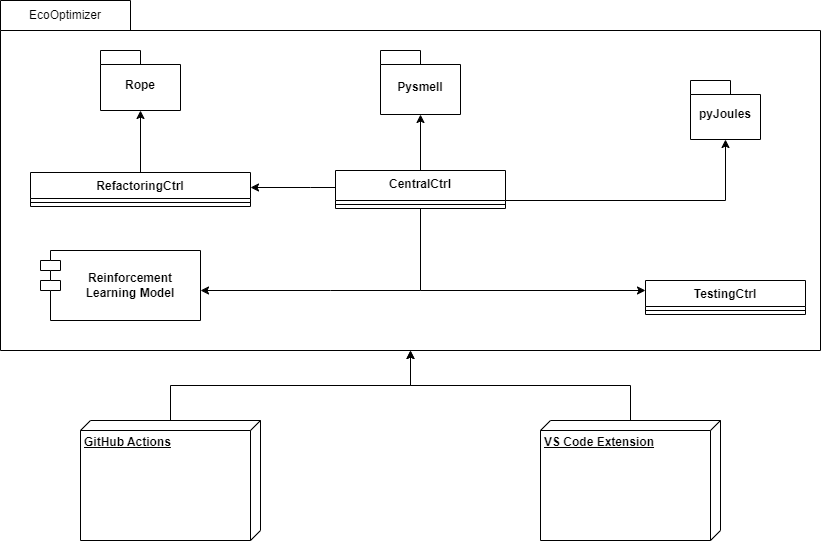
\includegraphics[width=\textwidth]{../Images/business-data-model.png}
  \caption{Business Data Model of System}
  \label{img:bdata-model}
\end{figure}

\newpage
\subsection{Data Dictionary}
\hyperref[tab:data-dict]{Table 3} shown below defines each component
in the system, including its attributes, type, and purpose. It
ensures clarity and consistency in data handling and serves as a
reference for development and testing.

% \renewcommand{\arraystretch}{1}
\begin{longtable}[H]{
    >{\raggedright\arraybackslash}p{3.5cm}
    >{\raggedright\arraybackslash}p{9cm}
  >{\raggedright\arraybackslash}p{2cm}}
  \toprule
  \textbf{Name} & \textbf{Content} & \textbf{Type} \\
  \midrule
  \endhead
  \bottomrule
  \caption{Data Dictionary for the System}
  \label{tab:data-dict}
  \endlastfoot

  ecooptimizer & Controller + Analysis + Refactoring + Energy
  Measurement & package \\ \midrule
  IDE extension & A plugin containing the \texttt{ecooptimizer}
  package delivered as an IDE extension & External Service Provider \\ \midrule
  Controller & Controlls the flow of execution within the package.
  Responsible for calling other modules and handling outputs & Module
  \\ \midrule
  Refactoring & Contains all necessary tools for refactoring the code
  smells defined in the package & Module \\ \midrule
  Energy Measurement & measures the energy consumption of the given
  source code & Module \\ \midrule
  Analysis & Contains all necessary tools for the analysis of the
  code smells defined in the package & Module \\
\end{longtable}

\section{The Scope of the Product}
This section outlines the boundaries and functionality of the
refactoring library, detailing what the system will and will not
deliver. It focuses on the internal components of the library, their
interactions, and how they collectively address the project's objectives.

\subsection{Product Boundary}
This subsection includes a diagram (\hyperref[img:prod-bound]{Figure
3}) showing the system's boundary, identifying its internal
components and their interactions. It clarifies what falls within the
scope of the product and what lies outside its responsibility.

\begin{figure}[H]
  \centering
  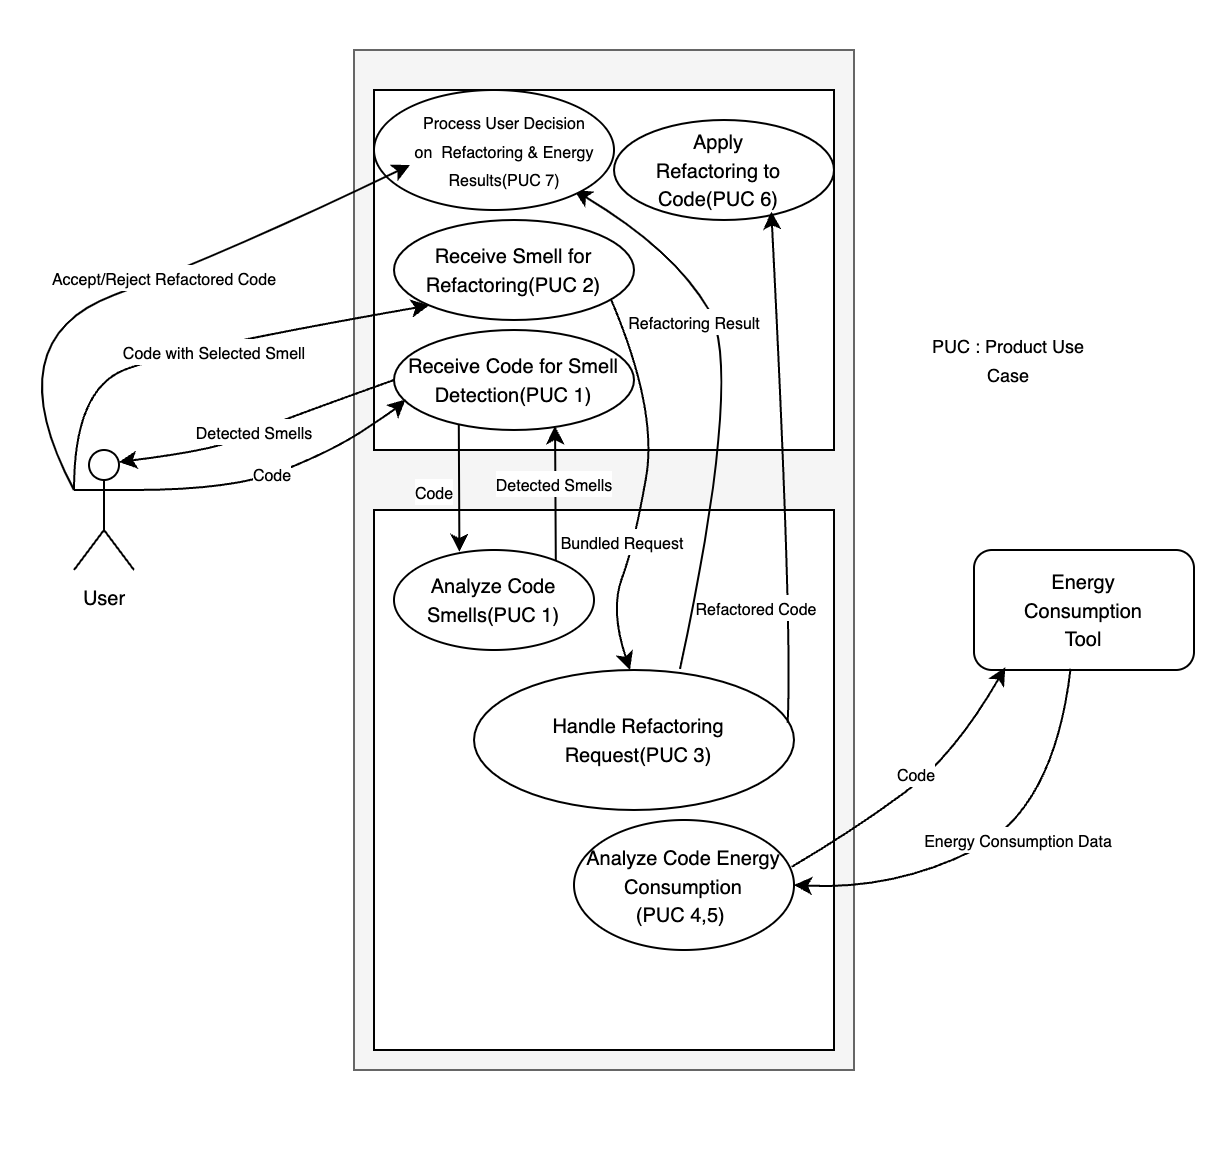
\includegraphics[width=0.9\textwidth]{../Images/use_case_diagram.png}
  \caption{Product Boundary Diagram of System}
  \label{img:prod-bound}
\end{figure}

\subsection{Product Use Case Table}
The following \hyperref[tab:puc]{table} summarizes the primary use
cases of the refactoring library, such as identifying code smells,
measuring energy consumption, applying refactorings, and allowing
users to accept or reject refactored code. Each use case briefly
describes the interaction between the user and the system.

\setlength\extrarowheight{2mm}

\begin{table}[H]
  \centering
  \renewcommand{\arraystretch}{0.85} 
  \begin{tabularx}{\textwidth}{|c|
      >{\raggedright\arraybackslash}X|
      >{\raggedright\arraybackslash}p{1.1in}| 
    >{\raggedright\arraybackslash}X|}
    \toprule \textbf{PUC \#} & \textbf{PUC Name} & \textbf{Actor/s} &
    \textbf{Input \& Output(s)} \\
    \midrule
    1 & Detect Code Smells & VS Code Plugin (via Refactoring Lib.) & Original Code (in), Identified Code Smells (out) \\
    2 & Toggle Smell Linting & User & Toggle Command (in), Enabled/Disabled Linting (out) \\
    3 & Filter Code Smells & User & Filter Criteria (in), Filtered Smells (out) \\
    4 & Configure Smell Detection & User & Threshold Parameters (in), Updated Detection Rules (out) \\
    5 & Select Code Smell & User & Selected Code Smell (in) \\
    6 & Refactor Code & VS Code Plugin (via Refactoring Lib.) & Code Segment (in), Refactored Code (out) \\
    7 & Measure Energy (Before) & Refactoring Library (via Energy Tool) & Original Code (in), Initial Energy Results (out) \\
    8 & Measure Energy (After) & Refactoring Library (via Energy Tool) & Refactored Code (in), Final Energy Results (out) \\
    9 & Show Results & VS Code Plugin & Refactored Code, Performance Metrics (out) \\
    10 & Accept/Reject Results & User & Refactored Code, Energy Results (in), Decision (out) \\
    11 & Clear Smell History & User & Clear Command (in), Reset Cache (out) \\
    12 & Access Documentation & User & Help Request (in), Documentation (out) \\
    13 & Generate System Logs & System & Log Request (in), Log File (out) \\
    \bottomrule
  \end{tabularx}
  \caption{Product Use Case Table of System}
  \label{tab:puc}
  \vspace{-2mm} 
\end{table}

\subsection{Individual Product Use Cases (PUC's)}
This subsection expands on the use cases listed in
\hyperref[tab:puc]{Table 4}, providing a detailed description of
each. It explains how the system components work together to fulfill
each use case, emphasizing expected functionality and outcomes for users.

\setlength{\parindent}{0pt}
\begin{enumerate}[label={\bf PUC \arabic*:}, wide=0pt, font=\itshape]

  \item \textbf{Detect Code Smells} \\[2mm]
    \textbf{Trigger:} The VS Code Plugin processes the input code
    using the refactoring library. \\[2mm]
    \textbf{Preconditions:}
    \begin{itemize}
      \item The VS Code Plugin has received the original code.
      \item The Refactoring Library is active and ready to analyze code.
    \end{itemize}
    \textbf{Actors:} VS Code Plugin (via Refactoring Library). \\
    \textbf{Outcome:} Code smells are identified and presented to the user. \\
    \textbf{Input:} Original Python Code. \\
    \textbf{Output:} List of detected code smells.

  \item \textbf{Select Code Smell for Refactoring} \\[2mm]
    \textbf{Trigger:} The user selects a detected code smell to be
    refactored. \\[2mm]
    \textbf{Preconditions:}
    \begin{itemize}
      \item The system has identified code smells.
      \item The user is reviewing the detected smells.
    \end{itemize}
    \textbf{Actors:} User. \\
    \textbf{Outcome:} The selected smell is sent to the refactoring tool. \\
    \textbf{Input:} Selected Code Smell. \\
    \textbf{Output:} Selected smell is marked for refactoring.

  \item \textbf{Refactor Code} \\[2mm]
    \textbf{Trigger:} The user has selected a code smell for
    refactoring. \\[2mm]
    \textbf{Preconditions:}
    \begin{itemize}
      \item Code smells have been detected.
      \item The user has selected a smell to refactor.
    \end{itemize}
    \textbf{Actors:} VS Code Plugin (via Refactoring Library). \\
    \textbf{Outcome:} The system refactors the selected code smell. \\
    \textbf{Input:} Code Segment. \\
    \textbf{Output:} Refactored Python Code.

  \item \textbf{Measure Energy Consumption Before Refactoring} \\[2mm]
    \textbf{Trigger:} The refactoring library submits the original
    code to the energy measurement tool. \\[2mm]
    \textbf{Preconditions:}
    \begin{itemize}
      \item The system has received the original code.
      \item The energy measurement tool is active and connected.
    \end{itemize}
    \textbf{Actors:} Refactoring Library (via Energy Measurement Tool). \\
    \textbf{Outcome:} Initial energy consumption is measured. \\
    \textbf{Input:} Original Python Code. \\
    \textbf{Output:} Initial Energy Consumption Results.

  \item \textbf{Measure Energy Consumption After Refactoring} \\[2mm]
    \textbf{Trigger:} The refactored code is submitted to the energy
    measurement tool. \\[2mm]
    \textbf{Preconditions:}
    \begin{itemize}
      \item The system has refactored the code.
      \item The energy measurement tool is active and connected.
    \end{itemize}
    \textbf{Actors:} Refactoring Library (via Energy Measurement Tool). \\
    \textbf{Outcome:} Final energy consumption is measured. \\
    \textbf{Input:} Refactored Python Code. \\
    \textbf{Output:} Final Energy Consumption Results.

  \item \textbf{Show Results} \\[2mm]
    \textbf{Trigger:} Refactored code and energy consumption metrics
    are ready. \\[2mm]
    \textbf{Preconditions:}
    \begin{itemize}
      \item The refactoring process has completed.
      \item Energy consumption before and after refactoring has been measured.
    \end{itemize}
    \textbf{Actors:} VS Code Plugin. \\
    \textbf{Outcome:} The refactored code and performance metrics are
    presented to the user. \\
    \textbf{Output:} Refactored Code, Energy Consumption Results.

  \item \textbf{Accept or Reject Refactoring Results} \\[2mm]
    \textbf{Trigger:} The user reviews the refactored code and its
    energy consumption results. \\[2mm]
    \textbf{Preconditions:}
    \begin{itemize}
      \item The system has presented the refactored code and energy
        consumption results.
    \end{itemize}
    \textbf{Actors:} User. \\
    \textbf{Outcome:} The user accepts or rejects the refactored
    code. If rejected, no changes are applied. If accepted, the
    refactored code replaces the original. \\
    \textbf{Input:} Refactored Code, Energy Consumption Results. \\
    \textbf{Output:} Accepted or Rejected Decision.

\end{enumerate}

\section{Functional Requirements}
\subsection{Functional Requirements}
\begin{enumerate}[label=FR \arabic*., wide=0pt, leftmargin=*]
  \item \emph{The system must accept Python source code files.}\\[2mm]
    {\bf Rationale:} The system needs to process Python code as its
    primary input to refactor and improve energy efficiency.\\
    {\bf Fit Criterion:} The system successfully processes valid
    Python files without errors and provides feedback for invalid files.\\
    {\bf Priority:} High
  \item \emph{The system must identify specific code smells that can
    be targeted for energy saving.}\\[2mm]
    {\bf Rationale:} Energy inefficiencies are often related to
    well-known code smells, so identifying them is the first step in
    improving efficiency.\\
    {\bf Fit Criterion:} The tool should be meet the SMELL\_COVERAGE
    for the detection and reporting of the following smells: Long
    Parameter List (LPL), Long Message Chain (LMC), Long Element
    Chain (LEC), Long Lambda Function (LLF), Complex List
    Comprehension (CLC), Member Ignoring Method (MIM), Cache Repeated Calls (CRC),
    String Concat in Loop (SCL).\\
    {\bf Priority:} High
  \item \emph{The system must suggest at least one appropriate
      refactoring for each detected code smell to decrease energy
    consumption or indicate that none can be found.}\\[2mm]
    {\bf Rationale:} For developers to optimize their code, the tool
    must provide an appropriate refactoring suggestion based on
    detected code smells.\\
    {\bf Fit Criterion:} The suggested refactored code demonstrates a
    measurable improvement in energy consumption as measured in kg.\\
    {\bf Priority:} High
  \item \emph{The system must produce valid refactored Python code as
    output or indicate that no possible refactorings were found.}\\[2mm]
    {\bf Rationale:} Refactored code must remain functional and
    error-free to ensure maintainability and usability.\\
    {\bf Fit Criterion:} The output code is syntactically correct and
    adheres to Python standards, validated by an automatic linter.\\
    {\bf Priority:} High
  \item \emph{The tool must require Python version 3.10 to run but
      must be capable of analyzing and refactoring Python code written
    for versions 3.8 and newer.}\\[2mm]
    {\bf Rationale:} The tool leverages features available in Python
    3.10 for its operation while ensuring compatibility with
    analyzing codebases written in Python 3.8 and 3.9, which are the
    most widely adopted recent major versions in use.\\
    {\bf Fit Criterion:} The tool operates correctly in a Python 3.10
    environment and successfully analyzes and refactors code written
    for Python versions 3.8, 3.9, and newer.\\
    {\bf Priority:} Medium
  \item \emph{The system must generate and display energy consumption metrics.}\\[2mm]
    {\bf Rationale:} Developers need clear metrics as a justification for energy efficient refactorings.\\
    {\bf Fit Criterion:} Energy consumption metrics are clear, well-structured, and
    provide actionable insights, allowing users to easily understand the results.\\
    {\bf Priority:} Medium
  \item \emph{The tool must provide comprehensive documentation and
    help resources.}\\[2mm]
    {\bf Rationale:} Detailed documentation is necessary to help
    users install, understand, and use the tool effectively.\\
    {\bf Fit Criterion:} Documentation covers installation, usage,
    and troubleshooting, receiving positive feedback for clarity and
    completeness from users.\\
    {\bf Priority:} Medium
  \item \emph{The system shall provide developers with refactoring
      suggestions within an IDE before changing code, allowing them
    to review and approve energy-efficient changes.}\\[2mm]
    {\bf Rationale:} Giving developers control over which
    refactorings are applied ensures that they can maintain the
    balance between energy efficiency and their coding style or
    project requirements.\\
    {\bf Fit Criterion:} The IDE plugin must display at least two
    refactoring options for inefficient code patterns, allowing
    developers to either apply or reject them before making any changes.\\
    {\bf Priority:} Medium
  \item \emph{The system shall provide developers with refactoring
      suggestions within an IDE before changing code, allowing them
    to review and approve energy-efficient changes.}\\[2mm]
    {\bf Rationale:} Giving developers control over which
    refactorings are applied ensures that they can maintain the
    balance between energy efficiency and their coding style or
    project requirements.\\
    {\bf Fit Criterion:} The IDE plugin must display at least two
    refactoring options for inefficient code patterns, allowing
    developers to either apply or reject them before making any changes.\\
    {\bf Priority:} Medium
  \item \emph{The system must allow users to filter detected code smells within the IDE plugin.}\\[2mm]
    {\bf Rationale:} Developers should be able to focus on specific types of inefficiencies based on their 
    project needs and priorities.\\
    {\bf Fit Criterion:} The plugin provides a user-friendly interface that enables filtering detected code 
    smells by category, severity, or type, ensuring a customized refactoring experience.\\
    {\bf Priority:} Medium
    \item \emph{The system should indicate code smells within a smell-linted file.}\\[2mm]
    {\bf Rationale:} Developers need a clear visual representation of detected code smells to efficiently identify problematic areas in their code.\\
    {\bf Fit Criterion:} The system highlights detected code smells within the source file, for example, by underlining or marking affected lines.\\
    {\bf Priority:} High

\item \emph{The system must allow for refactoring of specific smells.}\\[2mm]
    {\bf Rationale:} Developers should have the flexibility to refactor only selected code smells rather than applying all refactorings at once.\\
    {\bf Fit Criterion:} Users can click on a specific detected smell and choose to refactor only that issue.\\
    {\bf Priority:} High

\item \emph{The system must allow users to configure specific smell detection parameters.}\\[2mm]
    {\bf Rationale:} Different projects may have varying definitions of what constitutes a long lambda function or a long message chain, so customizable thresholds improve flexibility.\\
    {\bf Fit Criterion:} The system provides a configuration interface where users can set thresholds for smell detection (e.g., defining the maximum acceptable length for a lambda function or the number of chained method calls before triggering a warning).\\
    {\bf Priority:} Medium

\item \emph{The system should generate and allow users to access logs of system processes.}\\[2mm]
    {\bf Rationale:} Logs provide transparency on system operations, helping users debug issues and track changes.\\
    {\bf Fit Criterion:} The system generates logs detailing detected smells, applied refactorings, and system errors, accessible through an interface or log file.\\
    {\bf Priority:} Medium

\item \emph{The system must allow users to accept or reject suggested refactored changes and apply the corresponding action.}\\[2mm]
    {\bf Rationale:} Developers should have control over the changes made to their code to ensure refactorings align with project requirements.\\
    {\bf Fit Criterion:} The tool provides an interface where users can review, accept, or reject suggested refactorings before they are applied.\\
    {\bf Priority:} High

\item \emph{The system must allow users to toggle smell linting on and off within the IDE.}\\[2mm]
    {\bf Rationale:} Users should be able to control whether code smell detection is actively running, especially to avoid distractions in certain workflows.\\
    {\bf Fit Criterion:} The system provides a toggle button to turn smell linting on or off. When this is enabled, the tool automatically highlights smells in open files, and when disabled, all highlighting/indications are removed.\\
    {\bf Priority:} Medium

\item \emph{The system must allow users to remove the history of detected smells and other cached data.}\\[2mm]
    {\bf Rationale:} Clearing stored data helps users maintain a clean workspace, manage storage, and reset the tool for a fresh start.\\
    {\bf Fit Criterion:} The system provides an option to delete previously detected smells and cached data, ensuring a reset state when needed.\\
    {\bf Priority:} Medium

\item \emph{The system should allow for the enabling and disabling of specific smells for detection.}\\[2mm]
    {\bf Rationale:} Developers may want to focus on certain types of inefficiencies while ignoring others based on project-specific needs.\\
    {\bf Fit Criterion:} The system provides an interface where users can enable or disable specific code smells from being detected and reported.\\
    {\bf Priority:} Medium


\end{enumerate}

\section{Look and Feel Requirements}
\subsection{Appearance Requirements}
\begin{enumerate}[label=LFR-AP \arabic*., wide=0pt, leftmargin=*]
  \item \emph{The IDE plugin refactoring interface shall present the
      original and refactored code side by side, allowing developers to
    compare and choose between them easily.}\\[2mm]
    {\bf Rationale:} Providing a side-by-side view of the original
    and refactored code helps developers make informed decisions
    about applying changes.\\
    {\bf Fit Criterion:} The interface must display the original code
    on one side and the refactored code on the other, with clear
    options for developers to accept or reject the refactorings
    without confusion.\\
    {\bf Priority:} High
  \item \emph{The tool shall have a minimalist design, focusing only
    on essential elements to reduce clutter.}\\[2mm]
    {\bf Rationale:} A clean and simple interface allows developers
    to focus on the code and refactoring suggestions without
    distractions, improving usability.\\
    {\bf Fit Criterion:} The tool should prominently display only the
    code, refactoring suggestions, and energy metrics, omitting
    unnecessary visual elements or distractions.\\
    {\bf Priority:} Low
\end{enumerate}
\subsection{Style Requirements}
\begin{enumerate}[label=LFR-ST \arabic*., wide=0pt, leftmargin=*]
  \item \emph{The tool shall convey a professional and authoritative
    appearance to instill confidence in developers.}\\[2mm]
    {\bf Rationale:} A professional appearance helps build trust and
    encourages developers to use the tool confidently for
    energy-efficient refactoring.\\
    {\bf Fit Criterion:} After their first encounter with the tool,
    the amount of representative developers that feel that it is a
    trustworthy and reliable solution for energy-efficient
    refactoring should be above the MIN\_USER\_CONFIDENCE.\\
    {\bf Priority:} High
  \item \emph{The IDE plugin interface shall promote a calm and
      focused atmosphere, enhancing the developer's ability to
    concentrate on code improvements.}\\[2mm]
    {\bf Rationale:} A calm environment reduces distractions and
    improves productivity, allowing developers to focus on their work
    effectively.\\
    {\bf Fit Criterion:} Developers should report feeling less
    distracted and more productive while using the tool, with the
    amount of developers indicating a positive change in their coding
    environment meeting the MIN\_USER\_CONFIDENCE.\\
    {\bf Priority:} Medium
  \item \emph{The tool design shall be visually appealing and modern,
    aligning with contemporary software development tools.}\\[2mm]
    {\bf Rationale:} A modern design improves user experience and
    satisfaction, making the tool more enjoyable to use.\\
    {\bf Fit Criterion:} The number of users that express
    satisfaction with the tool's visual design and layout after their
    initial interaction should meet the MIN\_USER\_CONFIDENCE.\\
    {\bf Priority:} Medium
\end{enumerate}

\section{Usability and Humanity Requirements}
\subsection{Ease of Use Requirements}
\begin{enumerate}[label=UHR-EOU \arabic*., wide=0pt, leftmargin=*]
  \item \emph{The tool shall have an intuitive user interface that
    simplifies navigation and functionality.}\\[2mm]
    {\bf Rationale:} A simple, intuitive interface allows users to
    access the tool's key features quickly, improving usability and
    reducing the learning curve.\\
    {\bf Fit Criterion:} Users should be able to complete key tasks
    (e.g., parsing code, configuring settings) MAX\_TASK\_CLICKS limit.\\
    {\bf Priority:} High
  \item \emph{The tool shall provide clear and concise prompts for
    user input.}\\[2mm]
    {\bf Rationale:} Clear instructions help users understand what
    inputs are required, minimizing confusion and errors during the process.\\
    {\bf Fit Criterion:} The amount of test users that report that
    prompts are straightforward and guide them effectively through
    the process should meet the MIN\_USER\_EOU.\\
    {\bf Priority:} High
\end{enumerate}

\subsection{Personalization and Internationalization Requirements}
\begin{enumerate}[label=UHR-PSI \arabic*., wide=0pt, leftmargin=*]
  \item \emph{The tool shall allow users to enable or disable detection of individual code smells.}
  \\[2mm]
  {\bf Rationale:} Developers should be able to focus on relevant code smells for their specific project needs.\\
  {\bf Fit Criterion:} Users can successfully toggle detection of any smell type on or off.\\
  {\bf Priority:} High
  
  \item \emph{The tool shall allow users to customize highlight colors for each detected code smell type.}
  \\[2mm]
  {\bf Rationale:} Custom colors improve readability and accommodate different visual preferences.\\
  {\bf Fit Criterion:} Users can successfully change highlight colors for any smell type.\\
  {\bf Priority:} Medium
\end{enumerate}

\subsection{Learning Requirements}
\begin{enumerate}[label=UHR-LRN \arabic*., wide=0pt, leftmargin=*]
  \item \emph{The tool shall provide context-sensitive help that
    offers assistance based on the current user actions.}\\[2mm]
    {\bf Rationale:} Context-sensitive help ensures that users can
    receive timely and relevant assistance, reducing confusion and
    improving usability.\\
    {\bf Fit Criterion:} Help resources should be accessible within
    MAX\_TASK\_CLICKS limit.\\
    {\bf Priority:} High
  \item \emph{The tool shall have an available YouTube video
    demonstrating installation.}\\[2mm]
    {\bf Rationale:} Video tutorials provide visual learning
    resources that can make the installation process more accessible to users.\\
    {\bf Fit Criterion:} A YouTube video demonstrating installation
    should be present and easily accessible.\\
    {\bf Priority:} Low
\end{enumerate}

\subsection{Understandability and Politeness Requirements}
\begin{enumerate}[label=UHR-UPL \arabic*., wide=0pt, leftmargin=*]
  \item \emph{The tool shall communicate errors and issues politely
    and constructively.}\\[2mm]
    {\bf Rationale:} Polite and constructive error messages reduce
    frustration and enhance the user experience, making the tool more
    approachable.\\
    {\bf Fit Criterion:} User feedback should reflect that at least
    the MIN\_USER\_EOU of users perceive error messages as helpful
    and courteous, rather than frustrating or vague.\\
    {\bf Priority:} Medium
\end{enumerate}

\subsection{Accessibility Requirements}
\begin{enumerate}[label=UHR-ACS \arabic*., wide=0pt, leftmargin=*]
  \item \emph{The tool shall provide high-contrast colour themes to
    improve visibility for users with visual impairments.}\\[2mm]
    {\bf Rationale:} High-contrast themes ensure that visually
    impaired users can easily navigate and use the tool, enhancing
    accessibility.\\
    {\bf Fit Criterion:} Users should have access to at least 1 high
    contrast theme.\\
    {\bf Priority:} Low
\end{enumerate}

\section{Performance Requirements}
\subsection{Speed and Latency Requirements}
\begin{enumerate}[label=PR-SL \arabic*., wide=0pt, leftmargin=*]
  \item \emph{The tool shall analyze and detect code smells in the
    input code within a reasonable time frame.}\\[2mm]
    {\bf Rationale:} Fast analysis ensures that developers do not
    experience significant delays while reviewing code.\\
    {\bf Fit Criterion:} The tool should complete the analysis for
    files up to 1,000 lines of code in under SMALL\_FILE\_TIME, and
    for files up to 10,000 lines in under LARGE\_FILE\_TIME.\\
    {\bf Priority:} High
  \item \emph{The refactoring process shall be executed efficiently
    without noticeable delays.}\\[2mm]
    {\bf Rationale:} Fast refactoring ensures a smooth workflow for
    developers, preventing frustration during development.\\
    {\bf Fit Criterion:} The tool should refactor the code and
    generate output in under REFACTOR\_TIME for small to medium-sized
    files (up to 5,000 lines).\\
    {\bf Priority:} Medium
\end{enumerate}
\subsection{Safety-Critical Requirements}
\begin{enumerate}[label=PR-SCR \arabic*., wide=0pt, leftmargin=*]
  \item \emph{The tool shall ensure that no runtime errors are
      introduced in the refactored code that could result in data loss
    or system failures.}\\[2mm]
    {\bf Rationale:} Preventing runtime errors ensures system
    stability and reliability after refactoring.\\
    {\bf Fit Criterion:} The refactored code must produce valid Python code verified by the user upon accepting changes
    {\bf Priority:} High
\end{enumerate}
\subsection{Precision or Accuracy Requirements}
\begin{enumerate}[label=PR-PAR \arabic*., wide=0pt, leftmargin=*]
  \item \emph{The tool shall maintain the functionality of the
    original provided code in all its recommended refactorings.}\\[2mm]
    {\bf Rationale:} Ensuring functionality preservation is critical
    for refactorings to be reliable.\\
    {\bf Fit Criterion:} The tool should pass all tests from the
    user-provided test suite after refactoring, confirming that the
    original functionality remains intact.\\
    {\bf Priority:} High
  \item \emph{The tool shall reliably identify code smells with
    minimal false positives and negatives.}\\[2mm]
    {\bf Rationale:} High detection accuracy ensures that developers
    are not misled by incorrect or missed suggestions.\\
    {\bf Fit Criterion:} Detection accuracy should exceed
    DETECTION\_ACC when validated against a set of known cases.\\
    {\bf Priority:} Medium
  \item \emph{The tool shall produce valid refactored Python code as
    output or indicate that no possible refactorings were found.}\\[2mm]
    {\bf Rationale:} Ensuring that the tool produces valid output is
    essential for maintaining code quality.\\
    {\bf Fit Criterion:} The output code is syntactically correct and
    adheres to Python standards, validated by an automatic linter.\\
    {\bf Priority:} Medium
\end{enumerate}

\subsection{Robustness or Fault-Tolerance Requirements}
\begin{enumerate}[label=PR-RFT \arabic*., wide=0pt, leftmargin=*]
  \item \emph{The tool shall gracefully handle unexpected inputs,
    such as invalid code or non-Python files.}\\[2mm]
    {\bf Rationale:} Ensuring stability with error handling prevents
    tool crashes and improves user experience.\\
    {\bf Fit Criterion:} The tool should provide clear error messages
    and recover from input errors without crashing, ensuring stability.\\
    {\bf Priority:} High
  \item \emph{The tool shall have fallback options if a specific
    refactoring attempt fails.}\\[2mm]
    {\bf Rationale:} Providing fallback options ensures the tool
    remains functional even when a refactoring fails, reducing
    disruptions in development.\\
    {\bf Fit Criterion:} In the event of a failed refactoring, the
    tool should log the error and propose alternative refactorings
    without stopping the process.\\
    {\bf Priority:} Medium
\end{enumerate}

\subsection{Capacity Requirements}
\begin{enumerate}[label=PR-CR \arabic*., wide=0pt, leftmargin=*]
  \item \emph{The tool shall efficiently manage large codebases.}\\[2mm]
    {\bf Rationale:} Efficient handling of large projects ensures
    that the tool remains usable for teams working with extensive codebases.\\
    {\bf Fit Criterion:} The tool must process projects with up to
    100,000 lines of code within LARGE\_CODE\_BASE\_TIME, maintaining
    performance standards.\\
    {\bf Priority:} High
\end{enumerate}

\subsection{Scalability or Extensibility Requirements}
\begin{enumerate}[label=PR-SER \arabic*., wide=0pt, leftmargin=*]
  \item \emph{The tool shall be designed to allow easy addition of
    new code smells and refactoring methods in future updates.}\\[2mm]
    {\bf Rationale:} Extensibility ensures that the tool remains
    relevant and adaptable to future developments in coding standards
    and practices.\\
    {\bf Fit Criterion:} New code smells or refactorings can be
    incorporated with minimal changes to existing code, ensuring that
    current functionality remains intact.\\
    {\bf Priority:} Medium
\end{enumerate}

\subsection{Longevity Requirements}
\begin{enumerate}[label=PR-LR \arabic*., wide=0pt, leftmargin=*]
  \item \emph{The tool shall be maintainable and adaptable to future
    versions of Python and changing coding standards.}\\[2mm]
    {\bf Rationale:} Ensuring the tool can be updated easily
    guarantees that it will remain useful and relevant over time.\\
    {\bf Fit Criterion:} The codebase should be well-documented and
    modular, facilitating updates with minimal effort.\\
    {\bf Priority:} Medium
\end{enumerate}

\section{Operational and Environmental Requirements}

The Operational and Environmental Requirements define the conditions
under which the system must function effectively. These requirements
ensure that the system performs reliably within specified operational
boundaries, such as compatibility, deployment, and environmental
constraints. Additionally, this section addresses the external
environmental factors that could influence the system. Meeting these
requirements is critical to ensure the tool’s proper operation and
sustainability in various working environments.

\subsection{Expected Physical Environment}

\begin{enumerate}[label=OER-EP \arabic*., wide=0pt, leftmargin=*]
  \item \emph{The product shall be used in temperatures ranging from
    \SI{10}{\celsius} - \SI{35}{\celsius}.}\\[2mm]
    {\bf Rationale:} A computer's safe operating range is
    \SI{10}{\celsius} - \SI{35}{\celsius} ~\citep{PCTemp}. If the
    computer doesn't work then it is not possible to use the
    refactoring library. \\
    {\bf Fit Criterion:} The computer turns on, and no temperature
    warning is issued. \\
    {\bf Priority:} High
  \item \emph{The product shall be used in proximity to a stable
    power supply.}\\
    {\bf Rationale:} As a coding library, the product depends on the
    continuing operation of the computer system it is used on. Should
    the computer lose power, the refactoring library will see its
    processes halted. \\
    {\bf Fit Criterion:} The computer is connected to a power outlet
    or the computer possesses charge on its battery. \\
    {\bf Priority:} High
\end{enumerate}

\subsection{Wider Environment Requirements}
\begin{enumerate}[label=OER-WE \arabic*., wide=0pt, leftmargin=*]
  \item \emph{The system must align with widely used emissions
      standards (e.g., GRI 305, GHG, ISO 14064)
    ~\citep{GHG,ISO14064,GRI305}.}\\[2mm]
    {\bf Rationale:} Providing metrics tailored to these standards,
    makes the library reporting tool more attractive to users part of
    companies looking to reduce their ecological footprint. \\
    {\bf Fit Criterion:} The emissions tracked by the standards are
    present in the reported metrics. \\
    {\bf Priority:} Medium
\end{enumerate}

\subsection{Requirements for Interfacing with Adjacent Systems}
\begin{enumerate}[label=OER-IAS \arabic*., wide=0pt, leftmargin=*]
  \item \emph{The library should be compatible with the Visual Studio
    Code (VSCode) IDE.}\\[2mm]
    {\bf Rationale:} Developers will be able to refactor code easily
    without leaving their working environment, therefore enhancing
    the accessibility and usability of the library.\\
    {\bf Fit Criterion:} An extension is available for installation
    in VSCode marketplace.\\
    {\bf Priority:} Medium
  \item \emph{The library should support importing existing codebases
      and exporting refactored code and energy savings reports in
    standard formats (e.g., JSON, XML)}\\[2mm]
    {\bf Rationale:} This ensures that users can easily integrate the
    library into their existing workflows without significant disruption.\\
    {\bf Fit Criterion:} Developers are able to refactor existing
    codebases and view relevant metrics.\\
    {\bf Priority:} Medium
\end{enumerate}

\subsection{Productization Requirements}
\begin{enumerate}[label=OER-PR \arabic*., wide=0pt, leftmargin=*]
  \item \emph{The library shall be package with PIP and made
    available to python users through the public package manager.}\\[2mm]
    {\bf Rationale:} As a widely used package manager, PIP will be
    able to distribute the library to any users that wish to use it.\\
    {\bf Fit Criterion:} Users are able to install the library using
    \texttt{pip install}. \\
    {\bf Priority:} Medium
\end{enumerate}

\subsection{Release Requirements}
\begin{enumerate}[label=OER-RL \arabic*., wide=0pt, leftmargin=*]
  \item \emph{All core functionalities specified in the requirements
      must be implemented and tested, including energy consumption
    measurement, automated refactoring, and reporting features.}\\[2mm]
    {\bf Rationale:} This will ensure that the library delivers the
    promised capabilities to users.\\
    {\bf Fit Criterion:} Follows the steps outlined in the
    Verification and Validation (V\&V) plan.  \\
    {\bf Priority:} Medium
  \item \emph{The library must be ready for release by March 17th, 2025.}\\[2mm]
    {\bf Rationale:} The library must be ready for final
    demonstration as a requirement of the McMaster University SFRWENG
    4G06 Capstone course.\\
    {\bf Fit Criterion:} The project is ready for the final
    demonstration of the appointed date.\\
    {\bf Priority:} Low
\end{enumerate}

\section{Maintainability and Support Requirements}
The following are defined as maintainability requirements:
\subsection{Maintenance Requirements}
\begin{enumerate}[label=MS-MNT \arabic*., wide=0pt, leftmargin=*]
  \item \emph{The tool must allow new refactoring techniques to be
    added within one week of identification.}\\
    {\bf Rationale:} Rapid integration of new techniques ensures the
    tool remains up-to-date with evolving best practices in
    energy-efficient coding.\\
    {\bf Fit Criteria:} Developers can integrate new refactoring
    methods into the tool, and they are fully operational within
    NEW\_REFACTOR\_TIME.\\
    {\bf Priority:} Medium

  \item \emph{The tool must be maintainable by developers who are not
    the original creators.}\\
    {\bf Rationale:} Ensuring that new developers can easily
    understand and modify the system reduces dependency on original
    developers and facilitates long-term maintenance.\\
    {\bf Fit Criteria:} Comprehensive documentation is available such
    as setup guides and code comments, allowing new developers
    to understand and modify the system within COMPREHENSION\_TIME.\\
    {\bf Priority:} High

  \item \emph{The tool must allow for easy rollback of updates in
    case of errors.}\\
    {\bf Rationale:} Quick rollback capabilities minimize downtime
    and user disruption in case an update introduces issues.\\
    {\bf Fit Criteria:} Any update can be reverted with minimal
    effort, ensuring the system returns to a stable state within
    ROLLBACK\_TIME.\\
    {\bf Priority:} Medium

  \item \emph{The tool must provide automated testing for all
    refactoring functions.}\\
    {\bf Rationale:} Automated testing ensures that changes do not
    introduce new bugs, maintaining the reliability and stability of the tool.\\
    {\bf Fit Criteria:} All refactoring methods have associated unit
    tests that run automatically with each code change, ensuring code
    coverage meets MIN\_CODE\_COVERAGE.\\
    {\bf Priority:} High

  \item \emph{Each version of the library must maintain compatibility
      with the current releases of external libraries during its
    development phase.}\\
    {\bf Rationale:} Keeping external libraries up-to-date ensures
    compatibility and leverages improvements or security patches
    provided by library maintainers.\\
    {\bf Fit Criteria:} The system successfully integrates updates
    from external libraries without breaking existing functionality.\\
    {\bf Priority:} Medium

\end{enumerate}

\subsection{Supportability Requirements}
This section is not needed for this project.

\end{enumerate}

\subsection{Adaptability Requirements}
\begin{enumerate}[label=MS-AD \arabic*., wide=0pt, leftmargin=*]
  \item \emph{The system must be compatible with the latest stable
    version of python (v3.13).}\\
    {\bf Rationale:} This allows the library to use the most
    up-to-date features, performance improvements, and security
    patches. Furthermore, it will ensure that users can integrate the
    library into modern projects without compatibility issues,
    reduces the risk of vulnerabilities.\\
    {\bf Fit Criteria:} The system passes all test cases when run in
    python 3.13.\\
    {\bf Priority:} High

  \item \emph{The system should offer backward compatibility with
    Python 3.10 and higher.}\\
    {\bf Rationale:} Offering backwards compatibility makes the
    library more accessible to users who may need to use the library
    in legacy codebases that can't easily be upgraded. Based on
    Python's versioning schedule, version 3.10 will not be considered
    end-of-life until nearly 2 years after the scheduled end of the
    development of this system.\\
    {\bf Fit Criteria:} All features of the system must work on
    Python 3.10 and higher versions, with minimal degradation in
    performance or functionality\\
    {\bf Priority:} Low

  \item \emph{The system must be able to detect and handle Python
    version-specific features and syntax.}\\
    {\bf Rationale:} Depending on the Python version of the source
    code, the refactorings should be made accordingly to not
    introduce compatibility errors.\\
    {\bf Fit Criteria:} The input source code should pass the given
    test cases.\\
    {\bf Priority:} High

  \item \emph{The energy measurement module must be adaptable to
    cloud-based systems.}\\
    {\bf Rationale:} Many modern applications are hosted and run in
    cloud environments so, it is essential for the energy measurement
    module to operate effectively in cloud-based systems. This
    ensures that developers can accurately measure the energy
    consumption of their cloud-hosted applications.\\
    {\bf Fit Criteria:} The energy consumption module returns usable
    statistics related to the energy consumption of the cloud-application.\\
    {\bf Priority:} Medium

  \item \emph{The system must be deployable in both cloud-based
    environments and on-premise infrastructures to meet different user needs.}\\
    {\bf Rationale:} Whether the system is being used locally or in
    the cloud, developers still need access to the features offered
    by the system. Some developers might not even host their
    applications, and, even if they do, they might want to conduct
    local testing. \\
    {\bf Fit Criteria:} The system should be fully functional in both
    cloud and local environments, with minimal configuration changes.\\
    {\bf Priority:} Medium

  \item \emph{The system must support major operating systems,
    including Windows, macOS, and Linux.}\\
    {\bf Rationale:} Developers may not all use the same operating
    system (OS), it's actually unlikely (even impossible) that they
    do. Allowing users to use the library on their preferred OS will
    only increase the adoption of the system.\\
    {\bf Fit Criteria:} The system must pass all tests on Windows
    10+, macOS 13+ (Ventura and later), and Linux distributions such
    as Ubuntu 22.04.5+ without requiring different codebases or
    significant modifications.\\
    {\bf Priority:} Low

  \item \emph{The system must provide seamless functionality across
    different versions of the same operating system.}\\
    {\bf Rationale:} Users do not adopt the latest version of an OS
    at the same rate and some programs are to complex or fragile to
    upgrade to newer systems.\\
    {\bf Fit Criteria:} The system runs without errors or crashes
    across multiple versions of Windows, macOS, and Linux, with no
    compatibility issues in handling file systems, dependencies, or libraries.\\
    {\bf Priority:} Low

  \item \emph{The system must offer consistent performance (e.g.,
      refactoring speed, energy consumption measurements) regardless of
    the underlying operating system.}\\
    {\bf Rationale:} Having the system be OS dependent would
    invalidate the point of being compatible with multiple OSes and
    conflict with requirement MS-AD 6.\\
    {\bf Fit Criteria:} Performance metrics, such as time taken for
    refactoring and energy measurements, must not vary by more than
    OS\_PERF\_DIFF\_LIMIT across different operating systems during testing.\\
    {\bf Priority:} Low

\end{enumerate}

\section{Security Requirements}
\subsection{Access Requirements}
\begin{enumerate}[label=SR-AR \arabic*., wide=0pt, leftmargin=*]
  \item \emph{The tool must be capable of protecting data during
    active sessions without requiring authentication of the user.}\\[2mm]
    {\bf Rationale:} Ensuring secure handling of data during
    processing eliminates the need for user authentication, thereby
    improving the tool's accessibility. Organizational code is
    already access-controlled for developers, therefore
    authentication is unnecessary for the tool.\\
    {\bf Fit Criterion:} The tool allows users to submit code and
    view refactoring results without requiring login credentials, and
    no sensitive data is stored beyond the active session.\\
    {\bf Priority:} High
  \item \emph{Only the refactoring tool can communicate with the
    energy consumption tool.}\\
    {\bf Rationale:} Energy consumption tool is an internal
    abstracted service that is not directly needed by the user.\\
    {\bf Fit Criterion:} The refactoring tool does not include any
    exposed API endpoints to the energy consumption tool.\\
    {\bf Priority:} High
\end{enumerate}
\subsection{Integrity Requirements}
\begin{enumerate}[label=SR-IR \arabic*., wide=0pt, leftmargin=*]
  \item \emph{The tool must prevent unauthorized, external changes to
    the refactored code and energy reports.}\\[2mm]
    {\bf Rationale:} The system must maintain code consistency and
    correctness of the original input and energy improvement data.
    Any corruption of the code could undermine trust in the tool.\\
    {\bf Fit Criterion:} The system must reject malformed data
    inputs, ensure data integrity during processing and transmission,
    and maintain comprehensive logging of system activities. It
    should safeguard against data corruption to maintain trust in the
    tool's outputs..\\
    {\bf Priority:} High
\end{enumerate}
\subsection{Privacy Requirements}
\begin{enumerate}[label=SR-PR \arabic*., wide=0pt, leftmargin=*]
  \item \emph{The tool must ensure that no personal user data, such
      as GitHub profile, commit history, working hours, or any
      identifiable information, is collected or stored during its
    operation. }\\[2mm]
    {\bf Rationale:} Personal information, including coding habits,
    working patterns, and associated data (such as GitHub profile or
    commits), is sensitive and must not be used to ensure that users
    maintain full control over their personal data.\\
    {\bf Fit Criterion:} The tool analyzes code and provides
    refactoring suggestions without collecting, storing or
    transmitting any personal information about the user.\\
    {\bf Priority:} High
  \item \emph{Any data related to user submissions, energy reports
      and refactored results must be treated as confidential and
    handled securely throughout processing and transmission.}\\
    {\bf Rationale:} The tool must ensure user trust by safeguarding
    all user submissions and related data against unauthorized access
    or tampering. Secure handling of data during active sessions
    maintains the integrity and reliability of the tool. \\
    {\bf Fit Criterion:} The system processes user submissions,
    energy reports, and refactored results securely within the active
    session. No data is stored or retained after processing, ensuring
    all user information remains private and protected.\\
    {\bf Priority:} High
\end{enumerate}
\subsection{Audit Requirements}
\begin{enumerate}[label=SR-AUR \arabic*., wide=0pt, leftmargin=*]
  \item \emph{The tool should maintain a log of operational events
      related to the refactoring process, including code detetction,
    energy analysis, and refactoring.}\\[2mm]
    {\bf Rationale:} The tool must ensure transparency in its
    operation by providing a record of key system actions, enabling
    the user to debug or review tool behavior.\\
    {\bf Fit Criterion:} The system generates a log of important
    operational events, such as the start and completion of analysis,
    energy measurements, and refactoring. \\[2mm]
    {\bf Priority:} Medium
  \item \emph{The tool should log user-triggered actions, such as
      code submissions and the initiation of refactoring processes,
    without storing any user-specific or identifiable data. }\\
    {\bf Rationale:} The tool must provide accountability for user
    interactions with the system, allowing the user to trace and
    verify the actions they have taken within the session.\\
    {\bf Fit Criterion:}  The system logs events such as user code
    submissions, requests for refactoring, and access to refactoring
    results. These logs do not include personal identifiable user data.\\
    {\bf Priority:} Medium
\end{enumerate}
\subsection{Immunity Requirements}
\begin{enumerate}[label=SR-AUR \arabic*., wide=0pt, leftmargin=*]
  \item \emph{The tool must minimize exposure to external threats,
      ensuring that the refactoring process is protected from
    unauthorized interference.}\\[2mm]
    {\bf Rationale:} Reducing reliance on external systems decreases
    vulnerability to external threats, such as malware or
    unauthorized access, and ensures a secure and reliable
    refactoring process.\\
    {\bf Fit Criterion:} The system operates without any external
    server communication so as exposure to external threats is
    limited. This setup inherently reduces exposure to external
    security risks.\\
    {\bf Priority:} High
\end{enumerate}

\section{Cultural Requirements}
The cultural requirements of this project include the following:
\subsection{Cultural Requirements}
\begin{enumerate}[label=CULT \arabic*., wide=0pt, leftmargin=*]
  \item \emph{The tool must avoid using colours or symbols that could
    be culturally sensitive or offensive.}\\
    {\bf Rationale:} Ensuring cultural sensitivity in design helps
    avoid alienating or offending users from diverse backgrounds,
    which is critical for global acceptance and usability.\\
    {\bf Fit Criteria:} Conduct a cultural review to ensure that all
    icons and colours used in the tool are neutral and universally acceptable.
    {\bf Priority:} Low


  \item \emph{The tool must not include content that could be
    considered culturally insensitive.}\\
    {\bf Rationale:} Avoiding culturally insensitive content ensures
    that the tool is respectful and inclusive, fostering a positive
    user experience across different cultures.\\
    {\bf Fit Criteria:} A cultural sensitivity review is conducted to
    ensure all content is appropriate for a global audience.
    {\bf Priority:} Medium

\end{enumerate}

\section{Compliance Requirements}
\subsection{Legal Requirements}
\begin{enumerate}[label=CR-LR \arabic*., wide=0pt, leftmargin=*]
  \item \emph{The system must respect user privacy by avoiding the
    collection of any personal or identifiable data.}\\[2mm]
    {\bf Rationale:} Ensuring privacy builds user trust and minimizes
    risks associated with handling sensitive information, even when
    specific privacy laws are not targeted.\\
    {\bf Fit Criterion:} The system avoids collecting or storing
    personal user data, including information about user activities
    and profiles, and operates entirely within the user’s local environment.\\
    {\bf Priority:} Medium
\end{enumerate}
\subsection{Standards Compliance Requirements}
\begin{enumerate}[label=CR-SCR \arabic*., wide=0pt, leftmargin=*]
  \item \emph{The system must conform to established Python coding
      standards and best practices for maintainability, readability and
    quality.}\\[2mm]
    {\bf Rationale:} Adhering to standards such as PEP 8 ensures the
    system’s codebase remains consistent, maintainable and compatible
    with coding standards, facilitating future development and collaboration.\\
    {\bf Fit Criterion:} The system implements static code analysis
    and adheres to Python coding standards, including PEP 8.\\
    {\bf Priority:} Medium
\end{enumerate}

\section{Open Issues}

This section outlines unresolved questions and challenges that may
impact the development, functionality, or integration of the system.
These issues require further research, discussion, or testing to
ensure successful project completion.\\

\begin{itemize}
  \item Further research is needed to determine the optimal balance
    between energy efficiency and code readability. While refactoring
    may improve energy consumption metrics, it could inadvertently
    make the codebase less maintainable and more difficult to expand
    in the long term.
  \item The same can be said when it comes to performance. More
    energy efficient code might actually end up being less efficient
    when it comes to time and space complexity.
\end{itemize}

\section{Off-the-Shelf Solutions}
\subsection{Ready-Made Products}

\begin{itemize}
  \item \textbf{Pylint:} A widely used static code analysis tool that
    detects various code smells in Python. It can be integrated into
    the refactoring tool to help identify inefficiencies in the code.
  \item \textbf{Flake8:} Linter that combines checks for style guide
    enforcement and code quality. Flake8 can assist in maintaining
    code standards while the tool focuses on energy efficiency.
  \item \textbf{PyJoule:} A tool for measuring the energy consumption
    of Python code. This product can provide essential data to
    evaluate the impact of refactorings on energy usage.
\end{itemize}

\subsection{Reusable Components}
\begin{itemize}
  \item \textbf{Rope:} A library for Python that provides automated
    refactoring capabilities, helping streamline the process of
    improving code quality.
\end{itemize}
\subsection{Products That Can Be Copied}
\begin{itemize}
  \item \textbf{SonarQube:} An open-source platform designed for
    continuous inspection of code quality. It helps developers manage
    code quality and security by analyzing source code to identify
    potential issues. Its architecture and methods for detecting code
    smells could be adapted to focus specifically on energy efficiency.
\end{itemize}

\section{New Problems}
\subsection{Effects on the Current Environment}
The introduction of the energy efficiency refactoring tool may lead
to several changes in the current development environment. These
effects include:
\begin{enumerate}
  \item The tool temporarily increases CPU and memory usage while
    running. The tool aims to optimize energy efficiency in code
    however it takes energy to run - in large codebases this could be
    significant energy and impact the performance of other
    applications running concurrently.
  \item The tool may have its own dependencies that now need to be
    included in the app or installed into the current system. Think
    Pysmells, Pyjoule etc.
\end{enumerate}

\subsection{Effects on the Installed Systems}
\begin{enumerate}
  \item Existing systems may need to be evaluated for compatibility
    with the new tool. Older versions of Python or other needed
    dependencies may not support the tool.
  \item The refactoring process could lead to variations in the
    performance of existing applications
  \item As the tool updates existing code, thorough testing will be
    needed to ensure everything still works correctly. This may
    require more effort from QA teams and additional time and
    resources to check the updated code.
\end{enumerate}

\subsection{Potential User Problems}
\begin{enumerate}
  \item Users may face difficulties in understanding how to
    effectively utilize the tool, particularly if they are not
    familiar with concepts like code smells and refactoring
    techniques. This learning curve may lead to initial frustration
    or reduced productivity.
  \item Some users may be resistant to adopting new tools or
    processes, particularly if they perceive the existing workflows
    as sufficient. This resistance could hinder the tool's successful
    implementation and limit its overall effectiveness.
  \item Users may misinterpret the output reports generated by the
    tool, such as energy savings or performance metrics. If users do
    not fully understand how to interpret these results, it could
    lead to incorrect conclusions about the tool's impact on their code.
  \item There is a risk that users might become overly reliant on the
    tool for refactoring without fully understanding the underlying
    principles. This could result in poor coding practices if users
    do not engage in thoughtful analysis of the suggested changes.
\end{enumerate}
\subsection{Limitations in the Anticipated Implementation Environment That May
Inhibit the New Product}
\begin{enumerate}
  \item \textbf{Limited Computational Resources:} Environments with
    restricted computational power may face challenges when running
    the tool, especially for large codebases. Limited resources could
    result in longer processing times or failures during analysis and
    refactoring.
  \item \textbf{Lack of Test Coverage:} If existing codebases lack
    comprehensive test suites, validating the functionality of
    refactored code may become challenging. Without adequate tests,
    it will be difficult to ensure that the tool's changes do not
    introduce new issues.
\end{enumerate}
\subsection{Follow-Up Problems}
\begin{enumerate}
  \item \textbf{Ongoing Maintenance:} The tool will need regular
    updates to stay compatible with new programming languages or
    standards, adding to the workload.
  \item \textbf{Performance Trade-offs:} Users may find that while
    some refactorings improve energy efficiency, they could
    negatively impact other performance metrics, such as execution speed.
\end{enumerate}
\section{Tasks}
\subsection{Project Planning}
\begin{itemize}

  \item \textbf{Development Approach}
    The team will use an agile development approach with the
    following high-level process:
    \begin{enumerate}
      \item Initial requirements gathering and product backlog creation
      \item Sprint planning and execution
      \item Regular testing and quality assurance
      \item Stakeholder reviews and feedback
      \item Iterative refinement
      \item Release planning and deployment
    \end{enumerate}

  \item \textbf{Key Tasks}
    \begin{itemize}
      \item Form cross-functional development team (already completed)
      \item Create initial product backlog and prioritize features
      \item Set up development environments and tools
      \item Establish CI/CD pipeline using GitHub Actions
      \item Develop core functionality:
        \begin{itemize}
          \item Determine code smells to address for energy-saving
          \item Implement code smell detection
          \item Develop appropriate refactorings for detected smells
          \item Measure energy consumption before and after refactoring
          \item Ensure original code functionality is preserved
        \end{itemize}
      \item Build out additional features iteratively
      \item Conduct regular testing (unit, integration, user acceptance)
      \item Refine based on stakeholder feedback
      \item Present final solution to stakeholders

    \end{itemize}
  \item \textbf{Timeline Estimate}
    \begin{itemize}
      \item Requirements Document (Revision 0): October 9th, 2024
      \item Hazard Analysis (Revision 0): October 23rd, 2024
      \item Verification \& Validation Plan (Revision 0): November 1st, 2024
      \item Proof of Concept: November 11th-22nd, 2024
      \item Design Document (Revision 0): January 15th, 2025
      \item Project Demo (Revision 0): February 3rd-14th, 2025
      \item Final Demonstration: March 17th-30th, 2025
      \item Final Documentation: April 2nd, 2025
      \item Capstone EXPO: TBD
    \end{itemize}

  \item \textbf{Resource Estimates}
    The team consists of 5 members who will all function as
    developers, sharing responsibilities for creating issues, coding,
    testing, and documentation.

  \item \textbf{Key Consideration}
    \begin{itemize}
      \item Data migration may be necessary for existing systems
      \item A phased development approach will help minimize major setbacks
      \item Regular stakeholder involvement will ensure alignment
        with business needs
    \end{itemize}

  \item \textbf{Documentation Process}
    \begin{itemize}
      \item Pull changes from \texttt{docs} (epic documentation branch)
      \item Create a working branch with format [main contributor
        name]/[descriptive topic]
      \item Commit changes with descriptive names
      \item Create unit tests for changes
      \item Create a pull request to merge changes into an epic branch
      \item Wait for all tests run with GitHub Actions to pass
      \item Wait for at least two approvals from teammates
      \item Merge changes into the target branch
    \end{itemize}

\end{itemize}

By following this agile approach and development process, the team
aims to deliver a high-quality product iteratively while maintaining
flexibility to adapt to changing requirements

\subsection{Planning of the Development Phases}

The planning of the development phases is based on the deliverables
submissions as follows:

\begin{enumerate}

  \item \textbf{Requirements Phase}
    \begin{itemize}
      \item Deliverable: Requirements Document (Revision 0)
      \item Due Date: October 9th, 2024
    \end{itemize}

  \item \textbf{Risk Assessment Phase}
    \begin{itemize}
      \item Deliverable: Hazard Analysis (Revision 0)
      \item Due Date: October 23rd, 2024
    \end{itemize}

  \item \textbf{Verification and Validation Planning}
    \begin{itemize}
      \item Deliverable: Verification \& Validation Plan (Revision 0)
      \item Due Date: November 1st, 2024
    \end{itemize}

  \item \textbf{Proof of Concept Implementation}
    \begin{itemize}
      \item Period: November 11th-22nd, 2024
    \end{itemize}

  \item \textbf{Design Phase}
    \begin{itemize}
      \item Deliverable: Design Document (Revision 0)
      \item Due Date: January 15th, 2025
    \end{itemize}

  \item \textbf{Initial Implementation and Demo}
    \begin{itemize}
      \item Deliverable: Project Demo (Revision 0)
      \item Period: February 3rd-14th, 2025
    \end{itemize}

  \item \textbf{Final Implementation and Testing}
    \begin{itemize}
      \item Deliverable: Final Demonstration
      \item Period: March 17th-30th, 2025
    \end{itemize}

  \item \textbf{Project Closure}
    \begin{itemize}
      \item Deliverable: Final Documentation
      \item Due Date: April 2nd, 2025
    \end{itemize}

  \item \textbf{Project Presentation}
    \begin{itemize}
      \item Event: Capstone EXPO
      \item Date: TBD
    \end{itemize}
\end{enumerate}

\section{Migration to the New Product}
\subsection{Requirements for Migration to the New Product}
The migration to the new tool will involve minimal disruption to
existing workflows, as the product is designed to integrate
seamlessly with Visual Studio Code. Developers will be able to
continue using their current workflows, with the addition of the
refactoring tool as a library that can be installed directly via
Python's package manager (pip) and an IDE plugin for an enhanced
development experience. The minimal installation and integration
requirements ensure ease of adoption for developers without needing
to overhaul existing infrastructure or processes.
\begin{itemize}
  \item \textbf{Installation Phase:}
    Developers can install the refactoring library directly using pip:
    \verb|pip install ecooptimizer|
    The IDE plugin can be installed by users through the Visual
    Studio Code marketplace.
  \item \textbf{Parallel Running:}
    There is no need for a phased implementation or parallel running
    of old and new systems. The tool can be directly integrated
    without affecting existing code or infrastructure.
  \item \textbf{Manual Backups:}
    Since the tool does not alter data but rather provides
    refactoring suggestions, no manual backups are required before installation.
  \item \textbf{Phased Rollout:}
    If required, developers can start using the refactoring library
    first, followed by the IDE plugin.
\end{itemize}
\subsection{Data That Has to be Modified or Translated for the New System}
Not Applicable

\section{Costs}
The total cost of developing this project is primarily based on the
effort involved by the development team, given that the tools and
platforms used (GitHub, open-source libraries) are free. The project
must be completed within the academic year (MVP ready by February
2025), which warrants smart planning and efficient resource allocation.

\subsection{Metrics for Estimation}
To estimate the total cost in terms of time and effort, the following
key metrics have been considered:
\begin{itemize}
  \item Number of input/output flows for the system.
  \item Number of business events.
  \item Number of product use cases.
  \item Number of functional and non-functional requirements.
  \item Number of constraint requirements.
\end{itemize}

\subsection{Estimation Approach}
Each deliverable has been assessed to estimate the time it will take
to implement based on the development environment. Early cost
estimates are based on general knowledge of the system and refined as
the team gradually gets a better understanding of the scope.

\subsection{Cost Breakdown}
\begin{itemize}
  \item \textbf{Development Effort:} Based on the team size and
    project timeline, following time allocation is estimated:
    \begin{itemize}
      \item Initial Research \& Setup: 50 hours per team member.
      \item Core development (e.g., refactoring tool, plugin): 300
        hours per team member.
      \item Testing and debugging: 80 hours per team member.
      \item Documentation \& finalization: 100 hours per team member.
      \item \textbf{Total estimated effort:} 530 hours per team member.
    \end{itemize}

  \item \textbf{Tools and Software:}
    \begin{itemize}
      \item GitHub (for CI/CD): Free account, with no cost expected.
      \item Open-source libraries: No associated costs.
    \end{itemize}

  \item \textbf{Testing Environment:}
    \begin{itemize}
      \item The testing of the refactoring tool and energy
        consumption measurements is planned to be carried out using
        free tools on open source projects, with no additional cost expected.
    \end{itemize}

\end{itemize}

\subsection{Estimated Cost}
The above discussion indicates that the total effort will be
approximately 2650 team hours spread across the project phases. These
estimates could be refined using more detailed information as the
project progresses.
\section{User Documentation and Training}
\subsection{User Documentation Requirements}
\begin{enumerate}
  \item \textbf{User Manual}
    \begin{itemize}
      \item \textbf{Purpose:} Provide comprehensive guidance on how
        to use the refactoring library
      \item \textbf{Target Audience:} Software developers integrating
        the library into their projects
      \item \textbf{Content:} Installation instructions, API
        reference, usage examples, and best practices
    \end{itemize}

  \item \textbf{Technical Specification}
    \begin{itemize}
      \item \textbf{Purpose:} Detail the library's architecture,
        algorithms, and integration points
      \item \textbf{Target Audience:} Technical leads and architects
        evaluating the library
      \item \textbf{Content:} System design, performance
        characteristics, and technical limitations
    \end{itemize}

  \item \textbf{Quick Start Guide}
    \begin{itemize}
      \item \textbf{Purpose:} Enable rapid adoption and basic usage
        of the library
      \item \textbf{Target Audience:} New users looking to quickly
        implement the library
      \item \textbf{Content:} Concise setup instructions and simple
        usage examples
    \end{itemize}
\end{enumerate}

\subsection{Training Requirements}
For end-users, formal training is not required. The tool is designed to be simple and intuitive, 
with the assumption that primary users with experience in Python and software development will 
have the necessary technical expertise to use the library effectively. The refactoring library 
operates through clear, well-documented interfaces and requires minimal setup, allowing users to 
quickly incorporate it into their workflow without additional training.\\

Furthermore, the tool will come with comprehensive user documentation that includes step-by-step 
instructions on how to set up, integrate, and use the library within their existing development 
processes. This documentation will provide examples of common use cases and a clear explanation of 
the features of the tool, ensuring that users can get started easily and efficiently.

\section{Waiting Room}

This section lists potential features and enhancements that are not
critical for the initial release of the system but may be considered
for future updates. These ideas represent additional functionalities
that could improve the tool’s performance, user experience, or
integration with other systems.

\begin{enumerate}[label=WTRM \arabic*., wide=0pt, leftmargin=*]
  \item \emph{The IDE plugin must provide interactive tips and
    progress indicators to guide users during the refactoring process.}\\[2mm]
    {\bf Rationale:} This helps prevent user confusion during the
    refactoring process and enhances the user experience by providing
    clear, real-time feedback.\\
    {\bf Fit Criterion:} Tips and progress indicators display
    automatically when users initiate a refactoring action in the
    VSCode interface.\\
    {\bf Priority:} Medium
  \item \emph{The tool must provide automated error reporting with
    user consent.}\\[2mm]
    {\bf Rationale:} Automated error reporting helps developers
    quickly identify and address issues, improving the tool's
    reliability and reducing downtime with an option to include
    additional comments for context.\\
    {\bf Fit Criterion:} Users are prompted to send error reports
    when an issue occurs, \\
    {\bf Priority:} Medium
  \item \emph{The tool must allow users to define custom refactoring
    rules or preferences within the plugin.}\\[2mm]
    {\bf Rationale:} This would allow developers more flexibility and
    control, enabling them to apply refactorings that best suit their
    projects while maintaining energy efficiency.\\
    {\bf Fit Criterion:} Users can create a configuration file that
    describes their refactoring preferences.\\
    {\bf Priority:} High
  \item \emph{The tool should provide a dashboard that offers deeper
      insights into refactoring decisions, showing side-by-side
      comparisons of energy consumption before and after refactoring,
    along with performance metrics.}\\[2mm]
    {\bf Rationale:} This would help users better understand the
    impact of refactoring on both energy consumption and performance.\\
    {\bf Fit Criterion:} Users are able to access energy metrics for
    all their projects on a centralized platform.\\
    {\bf Priority:} High
  \item \emph{The tool show provide a plugin that integrates with
      multiple popular IDEs and syncs information across them through a
    centralized database.}\\[2mm]
    {\bf Rationale:} Supporting multiple IDEs allows developers to
    use the tool within their preferred coding environments,
    enhancing user experience and adoption.\\
    {\bf Fit Criterion:} Integration guides are provided for each
    supported IDE, with successful installation and functionality
    confirmed through user testing.\\
    {\bf Priority:} Low
  \item \emph{The refactoring library must be able to provide energy
      efficient refactorings for a wide variety of program languages
    (e.g., Java, C/C++, C\#, JavaScript, TypeScript, Go, Rust, etc.)}\\[2mm]
    {\bf Rationale:} Users around the world code projects in
    multitudes of languages depending on the context of their work.
    Being able to refactor in most popular languages would allow for
    the widespread usage of the tool.\\
    {\bf Fit Criterion:} The tool accepts and tailors code from the
    detected/specified language.\\
    {\bf Priority:} Low
  \item \emph{A reinforcement learning model must be developed to
      learn from the most energy-efficient refactorings and user
    preferences over time.}\\[2mm]
    {\bf Rationale:} The model must evolve to improve its refactoring
    suggestions by identifying patterns in energy-efficient code
    transformations and user preferences. By adapting its
    recommendations, the system will refine its ability to balance
    energy savings with maintainability and user preferences.\\
    {\bf Fit Criterion:} The reinforcement learning model is trained
    using gathered refactoring data and energy consumption
    measurement. Over multiple iterations, the model should improve
    its ability to predict refactorings that maximize energy
    efficiency while aligning with user choices.\\
    {\bf Priority:} Medium
  \item \emph{The reinforcement learning model for the tool should
    accept human feedback in the reinforcement learning process.}\\[2mm]
    {\bf Rationale:} This will allow users to guide the system's
    refactoring decisions based on developer expertise and
    preferences. Moreover, it will balance automated refactoring with
    human oversight to ensure that complex refactoring decisions
    align with the project's goals and constraints.\\
    {\bf Fit Criterion:} The language model accepts human feedback
    and incorporates it into its future decisions.\\
    {\bf Priority:} Medium
\end{enumerate}

\section{Ideas for Solution}
In this section, we capture various ideas for implementing the
project requirements. These ideas provide technical approaches and
methods for achieving the energy-efficient refactoring of Python code
through the refactoring tool and IDE integration. By capturing these
ideas now, we ensure that potential technical approaches are not lost
and can be referred to during the design and development phase.
\begin{itemize}
  \item \textbf{Refactoring Library Implementation via AST Parsing:}
    Use Python’s built-in \texttt{ast} (Abstract Syntax Tree) module
    to analyze code structure. The refactoring library can traverse
    the AST to detect inefficiencies and apply refactorings without
    modifying code functionality.
  \item \textbf{IDE Plugin for Refactoring – Leveraging VS Code API:}
    Build an extension for Visual Studio Code that hooks into the
    editor’s event system to provide real-time refactoring suggestions.
\end{itemize}

\newpage{}
\section*{Appendix --- Reflection}

\begin{enumerate}[wide=0pt, leftmargin=*]
  \item \textit{What knowledge and skills will the team collectively
    need to acquire to successfully complete this capstone project?}

    \begin{itemize}
      \item Learn how reinforcement learning works as well as how to
        incorporate it into our project.
      \item Understanding of Python's performance characteristics and
        common code smells
      \item Experience in using libraries like rope for automated
        refactoring and familiarity with integrating linters such as
        Pylint or Flake8 into the development workflow.
      \item Ability to develop algorithms that analyze and compare
        different refactoring strategies, using tools like PyJoule
        for energy profiling.
      \item Proficiency in JavaScript or TypeScript, as most VS Code
        extensions are developed using these languages.
    \end{itemize}

  \item \textit{(\textbf{team}) For each of the knowledge areas and
      skills identified in the previous question, what are at least two
    approaches to acquiring the knowledge or mastering the skill?}

    \begin{itemize}
      \item \textit{Learn how reinforcement learning works as well as
        how to incorporate it into our project.}
        \begin{itemize}
          \item Watch online courses on reinforcement learning.
          \item Read articles/books teaching reinforcement learning.
          \item Look through open source python projects that use
            reinforcement learning tools such as PyTorch or TensorFlow.
          \item Read through the documentation for reinforcement learning tools.
        \end{itemize}

      \item \textit{Understanding of Python's performance
        characteristics and common code smells.}
        \begin{itemize}
          \item Enrol in courses like Effective Python or Python
            Performance Optimization on platforms like Coursera, edX, or Udemy.
          \item Work on real-world projects or contribute to
            open-source Python projects. Regular code reviews with a
            focus on performance
            will help identify common code smells and inefficiencies.
        \end{itemize}

      \item \textit{Experience in using libraries like rope for
          automated refactoring and familiarity with integrating
        linters such as Pylint or Flake8 into the development workflow.}
        \begin{itemize}
          \item Set up a personal or team-based project that uses
            rope for refactoring and integrates linters (Pylint or
            Flake8). Experimenting with these tools in a real project
            will provide direct experience with their workflows and limitations
          \item Read through documentation for the tools.
          \item Follow comprehensive tutorials or attend workshops
            focused on Python tooling.
        \end{itemize}

      \item \textit{Ability to develop algorithms that analyze and
          compare different refactoring strategies, using tools like
        PyJoule for energy profiling.}
        \begin{itemize}
          \item Conduct research on energy-efficient algorithms and
            their application in Python refactoring. Experiment with
            PyJoule to analyze the energy impact of different code structures.
          \item Work under the guidance of a mentor or collaborate
            with experts in energy-efficient computing.
        \end{itemize}

      \item \textit{Proficiency in JavaScript or TypeScript, as most
        VS Code extensions are developed using these languages.}
        \begin{itemize}
          \item Practise by building simple VS Code extensions using
            JavaScript or TypeScript using tutorials on YouTube.
          \item Take online courses specifically tailored to
            JavaScript or TypeScript for extension development
        \end{itemize}

    \end{itemize}


\end{enumerate}

2. \textit{(\textbf{Individual}) Of the identified approaches, which
will each team member pursue, and why did they make this choice?}

\subsubsection*{Ayushi Amin Reflection}

\medskip

\begin{itemize}[label={}, wide=0pt, leftmargin=*]

  \item \textit{Learn how reinforcement learning works as well as how
    to incorporate it into our project.}

    I would choose looking through open-source Python projects that
    use reinforcement learning tools like PyTorch or TensorFlow. It
    lets me see real-world applications, understand how others are
    using reinforcement learning, and gives me concrete examples to
    work with, which helps me learn more effectively through hands-on
    experience.

  \item \textit{Understanding of Python's performance characteristics
    and common code smells.}

    I would go with practical experience, contributing to open-source
    projects, where I can directly apply performance optimizations
    and get feedback through code reviews. Real-world application
    will help cement these concepts better.

  \item \textit{Experience in using libraries like rope for automated
      refactoring and familiarity with integrating linters such as
    Pylint or Flake8 into the development workflow.}

    I would go for hands-on implementation in my projects. I learn
    best by doing, so I would set up a project where I can integrate
    rope for refactoring and Pylint or Flake8 for linting. This would
    give me a chance to really see how these tools fit into the
    development process, and I could refine my setup as I work.

  \item \textit{Ability to develop algorithms that analyze and
      compare different refactoring strategies, using tools like
    PyJoule for energy profiling.}

    I would prefer diving into the research around energy-efficient
    algorithms and then trying things out with PyJoule. I enjoy
    exploring new tools and methods, so experimenting with how
    different code changes affect energy use would be a good challenge for me.

  \item \textit{Proficiency in JavaScript or TypeScript, as most VS
    Code extensions are developed using these languages.}

    I like learning by creating, so I would build an extension right
    away. This way, I would get immediate experience with JavaScript
    and TypeScript while learning the VS Code extension framework.

\end{itemize}

\subsubsection*{Mya Hussain Reflection}
To advance my skills for the capstone project, I plan on deepening my
understanding of Python’s performance characteristics and common code
smells while leveraging my existing knowledge of Python. I plan to
read up on different potential code smells, detection methods and
possible refactoring remedies and immediately apply these insights to
help develop a proof of concept (POC) for our project. For mastering
refactoring tools like Rope and integrating linters such as Pylint
and Flake8, I will set up a local project environment to experiment
with these tools specifically for our POC. Additionally, I’ll explore
energy-efficient algorithms and use PyJoule to analyze how different
refactoring strategies impact performance in our specific context. To
enhance my proficiency in JavaScript or TypeScript for developing VS
Code extensions, I plan on watching online tutorials and perhaps take
an online Javascript/Typescript course as it has been a while since I
have been familiar with the syntax. I will also watch tutorials on
how to set up a VSCode extension as this project will be my first
time doing it. I'm very excited to start coding up a POC and move on
from the documentation stage. With every requirement we write the
team feels more and more pressure to make sure our idea will work.
It's hard to write so much about a product that doesn't yet exist
without having the proof that it can exist. Or at least my mind is
having a hard time writing so much about what currently is an empty repository.

\subsubsection*{Tanveer Brar Reflection}
\medskip

\begin{itemize}[label={}, wide=0pt, leftmargin=*]

  \item \textit{Learn how reinforcement learning works as well as how
    to incorporate it into our project.}

    I plan to watch online courses on reinforcement learning. I
    prefer learning visually whenever possible. Since this is a
    fairly new concept for me, I think online courses would be the
    best, providing a mix of lectures and self-assignments. A lot of
    courses also provide access to an online learning community which
    is perfect for a beginner like me.

  \item \textit{Understanding of Python's performance characteristics
    and common code smells.}

    For this, I will contribute to open source Python projects. Live
    projects are a good way to expose to practical coding challenges
    related to performance and code smells. It will also allow me to
    learn from more experience contributors and spot common code
    smells so that I can write scalable and efficient Python code.

  \item \textit{Experience in using libraries like rope for automated
      refactoring and familiarity with integrating linters such as
    Pylint or Flake8 into the development workflow.}

    I will follow comprehensive tutorials to get experience in using
    Rope for automatic refactoring. Comprehension tutorials provide
    guided experience with Python tooling, helping to explore
    features of tools like Rope, Pylint, and Flake8 in-depth.  The
    tutorials are structured, therefore helping to quickly gain
    familiarity with functionality and usage in real-world scenarios.

  \item \textit{Ability to develop algorithms that analyze and
      compare different refactoring strategies, using tools like
    PyJoule for energy profiling.}

    For this I will conduct research on energy-efficient algorithms
    and their application in Python refactoring. This will give me
    the option to follow a hands-on approach which allows for
    comparing different strategies and asses their energy consumption
    in multiple scenarios.

  \item \textit{Proficiency in JavaScript or TypeScript, as most VS
    Code extensions are developed using these languages.}

    For this I will practise building simple VS Code extensions using
    JavaScript or TypeScript through YouTube tutorials. It can help
    me gain hands-on experience with the languages in a real-world
    context. These practical exercises can be used to not only
    solidfiy my understanding of JavaScript/TypeScript but also
    familiarize me with how these languages are used to create
    functional VS Code extensions, enhancing both my coding skills
    and extension development proficiency.

\end{itemize}

\subsubsection*{Sevhena Walker Reflection}
\medskip

\begin{itemize}[label={}, wide=0pt, leftmargin=*]

  \item \textit{Learn how reinforcement learning works as well as how
    to incorporate it into our project.}

    For this topic, I plan on watching online courses and tutorials
    since it's a subject I have basically no experience in. Watching
    videos is the better option for me in this case since having
    someone explain the knowledge and providing examples will allow
    me to grasp the material faster.

  \item \textit{Understanding of Python's performance characteristics
    and common code smells.}

    I believe reading articles and going through documentation will
    be best for me for this topic. I already have a good base in
    programming and Python specifically so written documents will
    allow me to digest the new information at my own pace.

  \item \textit{Experience in using libraries like rope for automated
      refactoring and familiarity with integrating linters such as
    Pylint or Flake8 into the development workflow.}

    When it comes to libraries and modules, I tend to fare well by
    just reading the documentation and looking over code examples
    using those tools.

  \item \textit{Ability to develop algorithms that analyze and
      compare different refactoring strategies, using tools like
    PyJoule for energy profiling.}

    For this topic, experimentation will be my best option as it is
    not really a matter of learning something completely new but
    applying a new tool in a known environment.

  \item \textit{Proficiency in JavaScript or TypeScript, as most VS
    Code extensions are developed using these languages.}

    I already have some experience working with those languages, so I
    will only need to refer to the documentation for the occasional
    refresher on syntax and such.

\end{itemize}

\subsubsection*{Nivetha  Reflection}
\medskip

\begin{itemize}[label={}, wide=0pt, leftmargin=*]

  \item \textit{Learn how reinforcement learning works as well as how
    to incorporate it into our project.}

    I prefer to look through open source Python projects that use
    reinforcement learning tools to get used to it. While
    documentation and tutorials are readily available online whenever
    I need to reference them, I’m interested in seeing how tools such
    as PyTorch are applied in a live project so that I can get a
    clear understanding of their use. If possible, I will also
    contribute to these open source projects to implement these tools
    in a side project before doing for the capstone. This way I can
    be ready to implement in our project.

  \item \textit{Understanding of Python's performance characteristics
    and common code smells.}

    I will enrol in online courses since they include structured
    learning for these tools to optimize Python code. These courses
    also include hands on exercises that I can practice solidifying
    my skills for identifying performance bottlenecks and avoiding code smells.

  \item \textit{Experience in using libraries like rope for automated
      refactoring and familiarity with integrating linters such as
    Pylint or Flake8 into the development workflow.}

    I plan to follow comprehensive tutorials as these can break down
    complex topics into manageable subtopics, therefore helping in
    gradually building experience in these libraries. I can follow
    them at my own pace, so I have time to both experiment and
    troubleshoot. This way I can fully grasp the process of
    integrating these into Python projects.

  \item \textit{Ability to develop algorithms that analyze and
      compare different refactoring strategies, using tools like
    PyJoule for energy profiling.}

    I plan to conduct research on analyzing the energy impact on
    various code structures using PyJoules. This way I can gather
    data to make informed refactoring decisions. This also opens up
    the opportunity to develop more efficient algorithms that can
    optimize performance and energy usage in Python applications.

  \item \textit{Proficiency in JavaScript or TypeScript, as most VS
    Code extensions are developed using these languages.}

    Taking online courses tailored to JavaScript or TypeScript for
    extension development would give me a deeper understanding of how
    these languages are used in developing VS Code extensions. These
    focused courses include key concepts and best practices, helping
    me quickly become comfortable  in the exact skills needed for
    extension development.

\end{itemize}

~\newpage

\bibliographystyle {plainnat}
\bibliography{../../refs/References}

\end{document}
